% \documentclass[german,bachelor,ul]{webisthesis} % Weimar
% \documentclass[german,bachelor,fsu]{webisthesis} % Jena
\documentclass[english,bachelor,ul]{webisthesis} % Leipzig
%
% Non-default programme
% ---------------------
% \documentclass[english,master,buw]{webisthesis}\global\thesisprogramme{Human-Computer Interaction}
% \documentclass[english,master,buw]{webisthesis}\global\thesisfrontpagefaculty{Faculty of Civil Engineering/Faculty of Media}\global\thesisprogramme{Digital Engineering}
% \documentclass[german,bachelor,buw]{webisthesis}\global\thesisprogramme{Informatik\\Schwerpunkt Medieninformatik}
% \documentclass[german,bachelor,buw]{webisthesis}\global\thesisprogramme{Informatik\\Schwerpunkt Security and Data Science}
%
% When you change the language, pdflatex may halt on recompilation.
% Just hit enter to continue and recompile again. This should fix it.


%
% Values
% ------
\ThesisSetTitle{Investigating Core Set-based Active Learning for Text Classification}
\ThesisSetKeywords{Active Learning, Text Classification, Dimensionality Reduction, Core-Set, t-SNE} % only for PDF meta attributes
\ThesisSetLocation{Leipzig} 

\ThesisSetAuthor{Yannick Brenning}
\ThesisSetStudentNumber{3732848}
\ThesisSetDateOfBirth{27}{8}{2002}
\ThesisSetPlaceOfBirth{Bamberg}

% Supervisors should usually be Professors from the candidate's university. A second supervisor is not always needed. 
\ThesisSetSupervisors{Prof. Dr. Martin Potthast,Christopher Schröder,Christian Kahmann}

\ThesisSetSubmissionDate{26}{4}{2024}

%
% Suggested Packages
% ------------------
\usepackage[sort&compress]{natbib}
%   Allows citing in different ways (e.g., only the authors if you use the
%   citation again within a short time).
%
\usepackage{booktabs}
%    For tables ``looking the right way''.
%
% \usepackage{tabularx}
%    Enables tables with columns that automatically fill the page width.
%
% \usepackage[ruled,algochapter]{algorithm2e}
%    A package for pseudo code algorithms.
%
\usepackage{algorithm}
%\usepackage{algorithm2e}
\usepackage{algpseudocode}
\usepackage{amsmath}
%    For tabular-style formatting of mathematical environments.
%

\usepackage{fontawesome}
\usepackage{float}
%    For lots of awesome glyphs: https://mirror.physik.tu-berlin.de/pub/CTAN/fonts/fontawesome/doc/fontawesome.pdf

\usepackage{multirow}
\usepackage{pdfpages}
\usepackage{pbox}
\usepackage{rotating}
\usepackage{graphicx}

%
% Commenting (by your supervisor)
% -------------------------------
\usepackage{xcolor}
\usepackage{soul}
\usepackage[width=1\textwidth]{caption}
\newcommand{\bscom}[2]{%
  % #1 Original text.
  % #2 Replacement text.
    \st{\scriptsize\,#1}{\color{blue}\scriptsize\,#2}%
  }

% Create links in the pdf document
% Hyperref has some incompatibilities with other packages
% Some other packages must be loaded before, some after hyperref
% Additional options to the hyperref package can be provided in the braces [], like in
% \usehyperref[backref] % This will add back references in the bibliography that some people like ... some don't ... so better ask your supervisor ;-)
\usehyperref

\renewcommand{\algorithmicrequire}{\textbf{Input:}}
\renewcommand{\algorithmicensure}{}

\begin{document}
\begin{frontmatter}
\begin{abstract}
This is the \LaTeX{} template for Bachelor and Master theses at Webis. This template contains several hints and conventions on how to structure a thesis, how to cite the work of others, and how to display your results besides plain text. 
\end{abstract}
\end{frontmatter}

\tableofcontents

\chapter{Introduction}

Text is one of the most widespread and important sources of information, but extracting data and tangible knowledge from it can be a difficult and expensive task. With the advent of the digital age, enormous amounts of unstructured texts have become available with more being generated by the day. Due to this increasingly large amount of textual data, manually processing information at a larger scale becomes infeasible and thus demands the use of computer-driven approaches. 

The classification of text, meaning the assignment of a category or class to a document or piece of text is one of the most common and useful ways to gain information from a piece of text. As the amount of available text content continues to grow, text classification tasks become an increasingly important area of research within the field of natural language processing. 

Thanks to machine learning and data science, many methods of extracting information from text have been developed with the purpose of performing text classification at a larger scale. This possibility for automated organization of data can enhance insights and decision-making across industries such as healthcare, finance, and social sciences, among many others. Active Learning (AL) is a subfield of machine learning in which the learning algorithm is able to perform queries on an information source in order to reduce the total amount of annotated data (\cite{settles.tr09}). This method can offer significant advantages in improving model performances and especially in reducing labeling costs. Though there is no universally optimal strategy, AL has been proven to be useful in many cases where annotating data is expensive or the total amount of data is very large (\cite{settles.tr09}). 

% One such model is the CNN (convolutional neural network), which is used in many recognition and learning tasks but needs to be trained on a large dataset. With AL, selecting the most effective data points to be labelled by the oracle from a large pool of unlabelled data can be a challenge, especially in the case of CNNs. 
Oftentimes, there is a large amount of unlabelled data available for an AL model to learn from. In this case, selecting the most effective data points to be labelled by the information source from this large pool becomes a crucial, but difficult challenge to overcome. 

One attempt at improving the effectiveness of AL in this regard is the Core-Set approach (\cite{DBLP:conf/iclr/SenerS18}). This method uses core-set selection to counter the issue of AL ineffectiveness on convolutional neural networks (\cite{DBLP:conf/iclr/SenerS18}). The proposed approach selects a set of points the pool such that a model learning over this subset can be consistent when provided the remaining data points. The method was shown to have improved results when compared to other approaches in the field of computer vision (\cite{DBLP:conf/iclr/SenerS18}, \cite{DBLP:conf/cvpr/CaramalauBK21}), which encompasses tasks that focus on enabling computers to interpret and understand visual information from the world. This field involves a variety of different methods including image classification, object detection, and semantic segmentation, all of which have significant importance in scientific research, classification tasks, and pattern recognition.

However, the Core-Set approach has been shown to have mixed results in cases of text classification using BERT (\cite{DBLP:conf/kdd/0002MM21}, \cite{DBLP:conf/emnlp/Ein-DorHGSDCDAK20}) and binary text classification using deep neural networks (\cite{DBLP:conf/cikm/Liu0LZW21}). In some cases, Core-Set performs poorly even when compared to the random sampling strategy (\cite{DBLP:conf/kdd/0002MM21}, \cite{DBLP:conf/aaai/ColemanCKCBBNSZ22}). Additional research suggests that the approach may even be less effective in computer vision tasks with higher numbers of classes as well as higher-dimensional feature spaces (\cite{DBLP:conf/iccv/SinhaED19}). The theoretical analysis shown in \cite{DBLP:conf/iclr/SenerS18} briefly mentions the potential issue of higher class numbers; however, it does not attempt to provide a potential solution to the problem.

The mixed results for Core-Set just mentioned motivated three different research questions for this thesis.

\begin{enumerate}
    \item Can we improve Core-Set's mixed results within the field of text classification using dimensionality reduction techniques?
    \item Does an uncertainty-based approach improve the performance of Core-Set?
    \item Can we balance the class distribution within the Core-Set selection, and how will this affect the learning process?
\end{enumerate}

% Particularly in first case, the experiments conducted on the Internal Dataset and TREC-6 show that Core-Set performs poorly when comparing the F1-scores to the random sampling strategy. 

% This thesis aims to explore the possibility of improving the Core-Set approach for text classification tasks. 

By first explaining Core-Set's functionality and the possible reasons for why it tends to underperform in certain classification tasks, I aim to then examine the performance of Core-Set in comparison to various baseline approaches on large datasets of text content in order to verify this claim. Furthermore, this thesis looks to modify and potentially improve the Core-Set approach for text classification with the previous three research questions in mind and demonstrate the results of these modifications as a part of its experiment.

In the following, Chapter 2 explains the background and related work on the topics of text classification (Section 2.1), active learning in general (Section 2.2), the Core-Set approach (Section 2.3), and dimensionality reduction (Section 2.4) more specifically. In Chapter 3, I describe my approach to modifying Core-Set for text classification using three general approaches. In Chapters 4 and 5, I present my experiment as well as show and discuss its results. Finally, Chapter 6 concludes the thesis and provides insights on potential future developments. 

\chapter{Background/Related Work}

This chapter first provides an overview of the fields of text classification and active learning, which are crucial for understanding Core-Set and its usage scenario within this thesis. I then give a brief review of Core-Set on both a conceptual and functional level. The concepts and notations introduced here will be necessary to understand the reasoning and functionality behind the following approaches employed in the experiment. Finally, this chapter outlines the field of dimensionality reduction, placing emphasis on techniques that will pertain to the subsequent chapters.

\section{Text Classification}

% **GENERAL**
Text classification is one of the most fundamental and important tasks in the field of Natural Language Processing (NLP). As a result, developing efficient automatic text classification methods has become an important research topic. 

% **APPLICATION**
One of the most common applications of text classification is determining whether the opinion associated with a certain document has a positive or negative sentiment, also known as sentiment analysis. This has a wide range of uses, including the possibility for businesses to better gauge customer opinions on products and services (\cite{DBLP:books/sp/mining2012/LiuZ12}) in order to adapt accordingly. This application is a binary classification task, meaning the classifier has two classes with which each document can be labelled (positive or negative). Similarly, one might apply this binary classification task to the problem of spam filtering in e-mails, text messages and more. 

Beyond that, many applications of text classification require multiple classes, such as news and content categorization. In this case, text classification algorithms can organize documents into specific topics or themes (e.g. Sports, Business, Politics, \dots) (\cite{DBLP:journals/csur/Sebastiani02}). Other applications include information retrieval, recommender systems, and document summarization (\cite{DBLP:journals/information/KowsariMHMBB19}).

% **PROCESS**
Generally, text classification methods can be divided into the following phases: data collection and preprocessing, feature extraction, classifier selection, and model evaluation (\cite{DBLP:journals/information/KowsariMHMBB19}, \cite{DBLP:journals/eswa/MironczukP18}, \cite{ikonomakis2005text}).

In the first stage, some form of text data necessary to complete some classification objective is acquired, ideally of a sufficient amount. Several open data sets are publicly available to this end (\cite{DBLP:conf/acl/PangL05}, \cite{DBLP:conf/nips/ZhangZL15}, \cite{DBLP:journals/nle/LiR06}). The preprocessing phase includes steps such as lemmatization, removal of stop words, tokenization and stemming. 

The preprocessed text data must them be converted into numerical feature vectors. There are a number of techniques for accomplishing this such as Bag-of-Words, TF-IDF (Term Frequency-Inverse Document Frequency), and word embedding methods such as Word2Vec or GloVe. In addition to the word embedding methods just mentioned which are known as static word embeddings, there exist context-sensitive methods as of the late-2010s such as BERT and ELMo (\cite{DBLP:conf/naacl/DevlinCLT19}, \cite{DBLP:conf/naacl/PetersNIGCLZ18}), which can better represent the varied senses encompassed by words depending on their contexts.

The next phase, classifier selection, is one of the most crucial steps in the text classification pipeline. Without a comprehensive grasp of the underlying concepts of each algorithm, we cannot effectively determine an appropriate model for the task. Commonly known algorithms include Logistic Regression, Na\"ive Bayes and Support Vector Machines. More recently deep learning models such as Convolutional Neural Networks (CNNs), Recurrent Neural Networks (RNNs) and Transformer Models have become established as state-of-the-art approaches, especially when considering large text classification tasks (\cite{chen2015convolutional}, \cite{DBLP:conf/ijcai/LiuQH16}, \cite{DBLP:conf/aaai/LaiXLZ15}, \cite{DBLP:conf/naacl/DevlinCLT19}, \cite{DBLP:conf/cncl/SunQXH19}). These different deep learning algorithms are increasingly popular due to their ability to model more complex and non-linear relationships within data (\cite{DBLP:journals/nature/LeCunBH15}). The Core-Set approach was also originally developed for the deep learning domain, more specifically CNNs. As a result, this thesis focuses on the use of deep learning models, specifically transformers.

Model evaluation is usually the ``final'' phase of the text classification process. This encompassees the assessment of the classifier's performance, for which a myriad of metrics such as accuracy, F1-score and AUC can be employed. Based on the evaluation, one can select a suitable model/strategy as well as attempt to optimize it, e.g. by tuning hyperparameters.

The process of text classification clearly includes many steps which can be optimized and examined. For this reason, going over the entire process in detail would exceed the scope of this thesis. With this in mind, this thesis' experiment does not focus on the initial steps such as data collection, preprocessing and feature extraction, but rather the model training and evaluation steps.

% **CHALLENGES(?)**

\section{Active Learning}

Active Learning has become an increasingly important field when considering the need for efficient model construction as well as the labelling bottleneck in various machine learning tasks. Many fields, such as speech recognition, information extraction and classification suffer from this bottleneck as a result of their instance labels being expensive or time-consuming to obtain (\cite{settles.tr09}). 

Generally, active learning takes place in one of three main scenarios, namely \textit{membership query synthesis}, \textit{stream-based selective sampling} and \textit{pool-based active learning}. 

In the case of membership query synthesis, a membership query is created in the form of some unlabelled instance from the original dataset (\cite{DBLP:journals/ml/Angluin87},\cite{DBLP:journals/ijon/WangHYL15}). In other words, this approach synthesizes a query \textit{de novo}, rather than selecting some query from the instance space. One challenge of this approach is ensuring that the synthesized query is consistent with meeting the constraints imposed by the real data. In the case of a human oracle, this can result in unrecognizable queries, for example in the case of computer vision tasks. Similarly, this issue could also apply to text classification, where the query synthesis produces unintelligible texts (\cite{langbaum92}, \cite{settles.tr09}).% TODO: Can I cite two papers for "essentially" the same definition (first one is the original paper, second one's explanation seemed more clear)

Stream-based selective sampling, in contrast, typically examines each unlabelled instance one at a time and decides whether to query the oracle or to assign a label (\cite{settles.tr09}).

Finally, we consider the pool-based approach as one of the commonly known applications of AL. This scenario assumes a large set of unlabelled instances and a small set of labelled instances, from which queries can be selectively drawn using a \textit{query strategy}. Generally, most approaches begin with some random selection of points to initialize the classifier. With each AL iteration, the query strategy selects new instances on which to train the classifier. This process is then repeated until some stopping criterion is met. 

The key difference to the stream-based approach is that pool-based learning considers the entire collection and attempts to select the most informative instances, as opposed to making individual query decisions. This can be useful in many real-world problems where plenty of unlabelled data is available and the pool is assumed to be closed (though this is not necessarily always the case) (\cite{settles.tr09}).

This thesis considers the case of the pool-based scenario, as does the original Core-Set paper. It is worth mentioning however, that Core-Set has also been applied in the stream-based context (\cite{DBLP:conf/icml/SaranYK0A23}).

\section{Core-Set}

The Core-Set approach as proposed by \cite{DBLP:conf/iclr/SenerS18} was originally designed for CNNs to tackle the problem of AL algorithms on large datasets. The empirical studies conducted by \cite{DBLP:conf/iclr/SenerS18} show that Core-Set outperforms other established query strategies when applied in the field of computer vision.

The task of AL is defined as a \textit{core-set selection} problem in which the algorithm selects a smaller subset of points with increased diversity to learn from such that the model can be competitive over a larger dataset. This problem ends up being equivalent to the \textit{k-Center} problem (\cite{DBLP:conf/iclr/SenerS18}), which is also referred to as the minimax facility location problem. 

In mathematical terms, given a set of points $ N $ and a budget $ k \leq |N| $, $k$-Center finds a subset $ \mathbf{s} \subseteq N $ of $ k $ points such that the maximum distance of any point in $ N \setminus \mathbf{s} $ to its closest center in $ \mathbf{s} $ is minimal (\cite{har2008geometric}). Core-Set applies this concept to the field of AL in that the $ k $ centers selected from $ N $ will be the instances selected to be labelled by our oracle.

Another way of viewing this problem is by placing circles around the points in our set of centers. If we denote the maximum distance of any point in $ N $ to its nearest center in $ \mathbf{s} $ with $ \delta_{\mathbf{s}} $ and we place circles with a $ \delta_{\mathbf{s}} $-radius around each center in $ \mathbf{s} $, we can ``cover'' the entire set of points $ N $. In other words, $k$-Center attempts to find the minimum $ \delta_{\mathbf{s}} $ such that all points lie within the union of the $ \delta_{\mathbf{s}} $-circles when placed upon each center (depicted in Figure~\ref{fig:coreset}). Due to the nature of k-Center, the selected points tend to be spread out throughout the dataset in order to ``cover'' all the unselected points, making this a diversity-based approach. 

\begin{figure}[htbp]
    \centering
    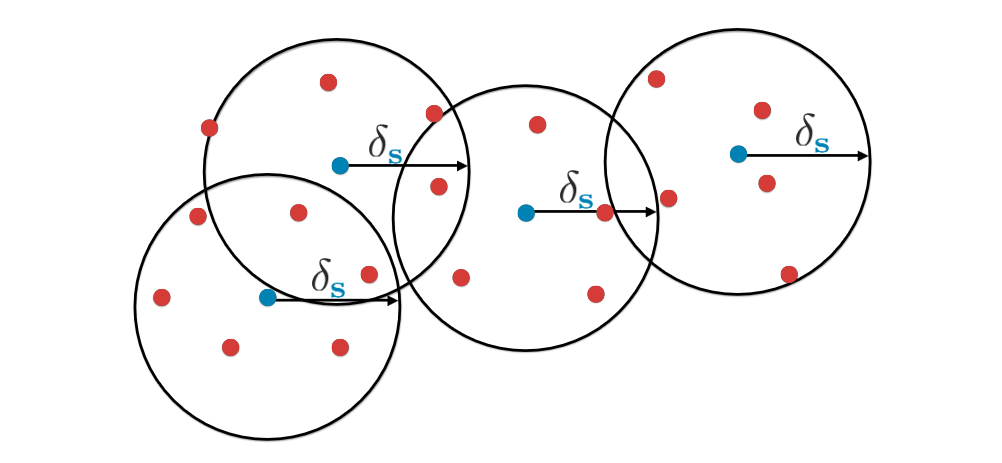
\includegraphics[width=1\textwidth]{img/core-set.png}
    \caption{Visualization of the k-Center approach from \cite{DBLP:conf/iclr/SenerS18}. $ \mathbf{s} $ denotes the set of $ k $ selected points, $ \delta_{\mathbf{s}} $ denotes the maximum distance of any point in $ N $ to its nearest center in $ \mathbf{s} $.}
    \label{fig:coreset}
\end{figure}

This problem has been shown to be NP-hard (\cite{DBLP:journals/dam/HsuN79}, \cite{DBLP:journals/anor/Hochbaum84}). As a result, Core-Set uses a greedy approach to solve the k-Center problem. However, it is worth noting that any approximation of k-Center is bound by twice the optimal solution (\cite{DBLP:journals/dam/HsuN79}). Let $ OPT $ denote the maximum distance of a center to a point in the optimal solution to k-Center, meaning the solution where $\delta_{\mathbf{s}} $ is minimal. Then the greedy approximation's resulting maximum distance $ \delta_{\mathbf{s}} $ to any center in $ \mathbf{s} $ is at the worst $ 2 \cdot OPT $ (\cite{mountkcenter}). The pseudocode used by \cite{DBLP:conf/iclr/SenerS18} for k-Center greedy within the active learning context can be seen in Algorithm~\ref{alg:coreset}.

\begin{algorithm}[htpb]
    \caption{k-Center-Greedy (adopted from \cite{DBLP:conf/iclr/SenerS18})}%
%\makeatletter\def\@currentlabel{CS}\makeatother
\label{alg:coreset}
\begin{algorithmic}


\Require data $ \mathbf{x}_i $, existing pool $ \mathbf{s}^0 $, budget $ b $
\State Initialize $ \mathbf{s} = \mathbf{s}^0 $
\Repeat
\State $ u = \text{argmax}_{i \in [n] \setminus \mathbf{s}} \text{min}_{j \in \mathbf{s}} \Delta(\mathbf{x}_i, \mathbf{x}_j) $
\State $ \mathbf{s} = \mathbf{s} \cup \{u\} $
\Until{$ |\mathbf{s}| = b + |\mathbf{s}^0|$}

\State \textbf{return} $\mathbf{s} \setminus \mathbf{s}^0 $
\end{algorithmic}
\end{algorithm}

The original paper by \cite{DBLP:conf/iclr/SenerS18} attempts to further improve the robustness of this approximation by placing an upper limit on the number of outliers that can be selected. This thesis focuses on and uses the regular k-Center greedy algorithm, which is generally better established due to ease of implementation and interpretability.

\section{Dimensionality Reduction}

% ADD STUFF HERE

As pointed out earlier, one of the major challenges of the Core-Set approach is handling data points with a higher dimensionality (\cite{DBLP:conf/iccv/SinhaED19}). Broadly speaking, this is a phenomenon coined by Richard E. Bellman known as the \textit{curse of dimensionality} (\cite{franccois2007high}). 
% NOT REALLY AS A RESULT...
As a result, many algorithms have been developed to transform data from a high-dimensional space into a low-dimensional space. This task directly poses another challenge: managing to reduce the dimensionality of the data while still being able to retain the highest possible amount of information. 

One such method is the Principal Components Analysis (PCA), which is one of the most popular linear techniques for dimensionality reduction (\cite{van2009dimensionality}). In essence, PCA linearly transforms the data into a representation that attempts to closely describe the variance of the initial data (\cite{jolliffe2016principal}). Other commonly used linear techniques include Linear Discriminant Analysis (LDA), Multidimensional Scaling (MDS), and Non-negative Matrix Factorization (NMF).

These techniques can be powerful; however, they often miss important non-linear structures in high-dimensional data. Therefore, non-linear techniques have been developed such as Isometric Mapping (Isomap), t-distributed Stochastic Neighbor Embedding (t-SNE) and Uniform Manifold Approximation and Projection (UMAP). 

\subsection{t-distributed Stochastic Neighbor Embedding}

t-SNE is a relatively modern probablistic approach that has improved upon many other non-linear techniques in creating a single map that reveals structure on many different scales. In addition, it manages to reduce the tendency of Stochastic Neighbour Embedding (SNE) to crowd data points together at the center by using a different cost function (\cite{van2008visualizing}). 

First, it converts the high-dimensional Euclidean distances into conditional probabilities, such that similar data points are assigned higher probabilities and dissimilar data points are assigned very low probabilities. It then creates a similar probability distribution over the lower-dimensional map such that the \textit{Kullback--Leibler divergence} (a measure of how one probability distribution differs from another) is minimized. 

The caveat of this technique is that its efficiency on large datasets relies on a variant of the Barnes--Hut algorithm, which results in reductions only being possible to the two- or three-dimensional space (\cite{DBLP:journals/corr/abs-1301-3342}). Because of this drawback, the method is generally used for the visualization of high-dimensional data, for which a reduction to two- or three-dimensional spaces is ideal.

\subsection{Uniform Manifold Approximation and Projection}

UMAP exists within a similar vein to t-SNE, but offers important improvements in some areas. This technique models the data with a fuzzy topological representation using simplices, then attempts to find some low-dimensional projection with the closest possible equivalent fuzzy topological structure (\cite{DBLP:journals/corr/abs-1802-03426}). Another key difference is that UMAP accomplishes this projection by attempting to minimize the cross-entropy between the topological representations, whereas t-SNE uses the Kullback-Leibler divergence. 

This paper also elaborates that the resulting reductions are competitive with t-SNE in the field of visualization and offer superior runtime performances. In addition, there exists no computational restriction on the embedding dimension, as opposed to t-SNE. As a result, \cite{DBLP:journals/corr/abs-1802-03426} also mentions it as a useful tool not only for visualization, but for machine learning tasks in general.

% t-SNE plots are strongly influenced by the chosen hyperparameters however, and thus a good understanding for the influence of these parameters is important. Particularly \textit{perplexity}, a measure of the effective number of neighbours, has a complex effect on the resulting reductions. According to \cite{van2008visualizing}, typical values for perplexity are between 5 and 50 and larger/denser datasets often generally require higher perplexities (\cite{vanHomepage}). Other commonly adjusted parameters include the learning rate and number of iterations for the optimization.

\chapter{Approach}

The following chapter describes my approach to the subsequent experiment. The attempt to improve upon and modify Core-Set resulted in multiple different iterations of the original k-Center greedy algorithm, which I have grouped into three different categories. Each of these different categories is designed to address one of the three research questions central to this thesis. 

I will first outline the dimensionality reduction-based approach, considering the two different nonlinear techniques discussed previously. After that, I will present two uncertainty-based approaches which take pointwise probabilities into account. The final approach for the experiment will attempt to use class balancing in combination with Core-Set.

\section{Dimensionality Reduction-Based}

As mentioned, distance-based methods such as Core-Set can be ineffective in higher dimensions. To overcome this challenge, I propose the application of a non-linear dimensionality reduction technique on the training data before selecting new points using Core-Set. My aim with this is attempting to preserve any non-linear structures within the datasets. In essence, this would modify the original $k$-Center greedy approach in that the distances computed between the points in $ \mathbf{s} $ and the unselected points would be different, since the algorithm would take in reduced embeddings (this modification is noted in Algorithm~\ref{alg:coreset-dr}).

\begin{algorithm}[htpb]
\caption{Dimensionality-Reduced $k$-Center-Greedy}%
%\makeatletter\def\@currentlabel{CS-TSNE}\makeatother
\label{alg:coreset-dr}
\begin{algorithmic}


\Require data $ \mathbf{x}_i $, existing pool $ \mathbf{s}^0 $, budget $ b $
\State Initialize $ \mathbf{s} = \mathbf{s}^0 $
\Repeat
\State $ u = \text{argmax}_{i \in [n] \setminus \mathbf{s}} \text{min}_{j \in \mathbf{s}} \Delta_{Reduced}(\mathbf{x}_i, \mathbf{x}_j) $
\Comment{Computing distances on}
\State $ \mathbf{s} = \mathbf{s} \cup \{u\} $
\Comment{reduced embeddings}
\Until{$ |\mathbf{s}| = b + |\mathbf{s}^0|$}

\State \textbf{return} $\mathbf{s} \setminus \mathbf{s}^0 $
\end{algorithmic}
\end{algorithm}

This resulted in two dimensionality-reduction based approaches. The first strategy, which I refer to as CS-tSNE, will use t-SNE in order to reduce the embeddings down to two dimensions. Additionally, I propose the use of UMAP as an alternative, which I will use to reduce the data to a 256-dimensional space.\footnote{Both of these approaches assume 768-dimensional embeddings.} This strategy will be referred to as CS-UMAP. 

\section{Uncertainty-Based}

Next, I will examine the effect of pointwise probabilities on the Core-Set algorithm. Core-Set currently operates using the distances between its points -- in this experiment, I propose an approach where Core-Set considers the probability distributions in addition to the distances. 

To accomplish this, I will be using an uncertainty-based approach. Uncertainty sampling, which was introduced by \cite{DBLP:conf/sigir/LewisG94}, essentially attempts to select the unlabelled examples with the lowest classification certainty. In this case, I specifically opted for an approach similar to that of Breaking-Ties (\cite{DBLP:journals/jmlr/LuoKGHSRH05}), where the instances with the smallest margin between their top two most likely classification probabilities are selected, essentially ``breaking the tie'' between the two most likely classes. In other words, if $ \mathbf{p}_{j, k}^* $ denotes the probability of the $ k $-th most likely class label for the $ j $-th instance, then Breaking-Ties seeks to select instances where $ \mathbf{p}_{j, 1}^* - \mathbf{p}_{j, 2}^* $ is minimal.

This approach resulted in two different implementation ideas: the first, which I will refer to as ``Weighted Core-Set'' (\ref{alg:wgc}), calculates the uncertainties prior to executing the standard Core-Set algorithm, then multiplies the resulting Core-Set distances and probabilities using weights (in this case, I used an 80--20 weighting in favour of the Core-Set distances). 

\begin{algorithm}[htpb]
\caption{Weighted k-Center-Greedy}%
\makeatletter\def\@currentlabel{WCS}\makeatother
\label{alg:wgc}
\begin{algorithmic}


\Require $ \mathbf{x}_i $, $ \mathbf{s}^0 $, $ b $, breaking-ties probabilities $ \mathbf{p}_{bt} $
\State Initialize $ \mathbf{s} = \mathbf{s}^0 $
\Repeat
\State $ d = \text{min}_{j \in \mathbf{s}} \Delta(\mathbf{x}_i, \mathbf{x}_j) $ 
    \State $ u = \text{argmax}_{i \in [n] \setminus \mathbf{s}} 0.8 \cdot d + 0.2 \cdot \mathbf{p}_{bt} $
    \Comment{Weigh results using linear}
\State $ \mathbf{s} = \mathbf{s} \cup \{u\} $
\Comment{combination}
\Until{$ |\mathbf{s}| = b + |\mathbf{s}^0|$}

\State \textbf{return} $\mathbf{s} \setminus \mathbf{s}^0 $
\end{algorithmic}
\end{algorithm}

The second, which I will call ``Re-ranked Core-Set'' (\ref{alg:rwgc}), opts to first compute a Core-Set twice the size of the original sample size $b$, then ``re-ranks'' the resulting distances according to Breaking-Ties uncertainties and finally selects the points with the $b$ highest uncertainties.

In theory, these two approaches aim to use uncertainties to improve Core-Set's selections such that the newly selected set of points should ideally contain instances which also have high uncertainties.

\begin{algorithm}[htpb]
\caption{Re-ranked k-Center-Greedy}%
\makeatletter\def\@currentlabel{RWCS}\makeatother
\label{alg:rwgc}
\begin{algorithmic}

\Require $ \mathbf{x}_i $, $ \mathbf{s}^0 $, $ b $, class probabilities $ \mathbf{p}_i $
\State Initialize $ \mathbf{s} = \mathbf{s}^0, r = \emptyset $
\Repeat
\State $ u = \text{argmax}_{i \in [n] \setminus \mathbf{s}} \text{min}_{j \in \mathbf{s}} \Delta(\mathbf{x}_i, \mathbf{x}_j) $
\State $ \mathbf{s} = \mathbf{s} \cup \{u\} $
\Until{$ |\mathbf{s}| = 2b + |\mathbf{s}^0|$}
\Comment{Compute Core-Set of size $2b$}

%\State $ \mathbf{p}_{bt} = \text{breaking\_ties}_{i \in \mathbf{s}}(\mathbf{p}_i) $

%\State $ \mathbf{s} = \mathbf{s} \cap \text{argpartition}(\mathbf{p}_{bt}, b) $

\Repeat
\State $ u = \text{argmin}_{j \in \mathbf{s} \setminus r}\mathbf{p}_{j, 1}^* - \mathbf{p}_{j, 2}^* $
\State $ r = r \cup \{u\} $
\Until{$ |r| = b $}
\Comment{Compute the $b$-highest BT-scores}

\State \textbf{return} $ r $
\end{algorithmic}
\end{algorithm}
\noindent $ \mathbf{p}_{j, k}^* $ denotes the probability of the $ k $-th most likely class label for the $ j $-th instance.

\section{Class Balance-Based}

Finally, I will take into account the class distributions within each Core-Set and select points based on the representation of each class. This approach will be called ``Class-Balanced Core-Set'' (\ref{alg:classbalanced}).

The basic idea with this approach is that the class distribution within out pool of labelled instances should, in theory, have an even class distribution such that the models learns from similar amounts of instances from each class. In other words, the query strategy (in this case Core-Set) should attempt to select more or less instances of a certain class depending on the discrepancy between the class distribution of the labelled pool and some balanced distribution of that class.

One way of determining the degree to which our pool of instances is ``class-balanced'' is by using the normalized entropy metric. This metric is based on the Shannon entropy $ H $ (\cite{DBLP:journals/bstj/Shannon48}), which is defined in Equation~\ref{eq:entropy} over some discrete random variable $ X $, which is in this case the class distribution.

\begin{equation}\label{eq:entropy}
    H(X) = -\sum_{x \in X} p(x) \log p(x)
\end{equation}

Dividing by the logarithm of the number of classes $n$ for the class distribution, we get the normalized entropy $ H_norm $(Equation~\ref{eq:nentropy}), also referred to as to as $ H_{REL} $ (\cite{wilcox1967indices}).

\begin{equation}\label{eq:nentropy}
    H_{norm}(X) = \frac{-\sum_{x \in X} p(x) \log p(x)}{\log n}
\end{equation}

This metric scales the output to lie between 0 and 1, such that 1 indicates a uniform distribution. This can be applied to the measurement of class imbalances, where a normalized entropy value closer to 1 indicates a more balanced class distribution and is thus a desirable result. 

To this end, I will divide a single query into multiple Core-Set computations, essentially constructing disjoint Core-Set selections for each class. For each class' Core-Set selection, the budget $ b $ (e.g., the amount of selected instances from this class) will depend on the desired class distribution.

First, the class distributions of the model's predictions and of the true labels are used to determine how many instances should ideally be queried for each class in order to achieve a ``balance'' in the labelled pool. In the corresponding pseudocode (\ref{alg:classbalanced}), this calculation has been denoted by the use of \texttt{target\textunderscore dist}, which uses an existing implementation from the Python library Small-Text (\cite{schroeder2023small-text}).

After this, $k$-Center greedy is used to select the desired number of points of each class, such that if $ k_i $ denotes the number of newly selected instances for the $ i $th class, then $ \sum_{c_i \in C} k_i = k $. 

\begin{algorithm}
    \caption{Class-Balanced k-Center Greedy}%
\makeatletter\def\@currentlabel{CB-CS}\makeatother
\label{alg:classbalanced}
\begin{algorithmic}

\Require $ \mathbf{x}_i $, $ \mathbf{s}^0 $, $ b $, true class labels $ y_i $, predicted class labels $ y^{pred}_i $ classes $ C $

\State $ d = \text{target\textunderscore dist}_{i \in [n] \setminus \mathbf{s}} (y_i, y^{pred}_i, C) $
\State Initialize $ \mathbf{s} = \mathbf{s}^0 $
\For{$c_i \in C$}
\Repeat
\State $ u = \text{argmax}_{i \in [n] \setminus \mathbf{s}} \text{min}_{j \in \mathbf{s}} \Delta(\mathbf{x}_i, \mathbf{x}_j) $
\State $ \mathbf{s} = \mathbf{s} \cup \{u\} $
\Until{$ |\mathbf{s}| = b + |\mathbf{s}^0|$}
\State $ \mathbf{s} = \mathbf{s} \cup \mathbf{s}_{c_i} $
\EndFor

\State \textbf{return} $\mathbf{s} \setminus \mathbf{s}^0 $
\end{algorithmic}
\end{algorithm}

\chapter{Experiment}

With these approaches in mind, this chapter will detail the experiment, first describing the data and setup of the experiment, and finally delving into its results. 

This experiment will take place within a simulated AL environment, meaning the oracle will not be a human expert or annotator, but rather an already labelled pool of data. To this end, I will select three established pre-labelled text classification datasets of different varieties. The AL will take place on these datasets using two different classifier models, each of which I will then combine with one of eight different query strategies. The query strategies to be compared will contain two baseline approaches, Core-Set itself, and the implementations of the previously discussed Core-Set variations. 

The following two sections will explain in greater detail the data and setup used as a basis for the conducted experiment. The performances will then be measured using two metrics, accuracy and AUC, throughout five runs for each combination of dataset, classifier and query strategy. In the final section, I will present and evaluate the experiment results.

\section{Data}

This experiment was conducted across three datasets commonly used in the field of text classification. These datasets are of three different types: sentiment analysis, questions, and news. 

For binary classification, I used \textbf{Movie Review}, a sentiment analysis dataset (\cite{DBLP:conf/acl/PangL05}) containing 5,331 positive and 5,331 negative online movie reviews. For multi-class text classification, I performed the AL on \textbf{AG's News} (\cite{DBLP:conf/nips/ZhangZL15}), a news dataset comprised of 120,000 training samples and 7,600 test samples, and \textbf{TREC} (\cite{DBLP:journals/nle/LiR06}), a question dataset containing 5,500 training samples and 500 test samples. The test set was provided in the case of AG's News and TREC, in the case of Movie Review I employed a split of the 10,662 samples myself, which can be seen alongside additional information in Table~\ref{tab:dataset-table}. Example instances from each dataset as well as their corresponding classes can also be seen in Table~\ref{tab:dataset-instances}.

\vspace{3\baselineskip}

\begin{table}[htpb]
    \centering
    \setlength{\tabcolsep}{16pt} % Adjust the spacing between columns
    \begin{tabular}{@{}lrrrr@{}} % use @{} to remove spacing; numbers should be right aligned
        \toprule
        % \multicolumn{4}{c}{\bfseries Some numbers}\\
        % \midrule
        \bfseries Dataset Name \scriptsize (ID) & \bfseries Classes & \bfseries Train & \bfseries Test & \bfseries MNC (*) \\
        % \cmidrule(l){2-4} % cmidrule: A line from 2nd to 4th column, trimmed on the left hand side
        \midrule
        Movie Review \scriptsize (MR) & 2 & 9,596 & 1,066 & 114.16 \\
        AG News \scriptsize (AGN) & 4 & 120,000 & 7,600 &  236.41 \\
        TREC \scriptsize (TREC) & 6 & 5,452 & 500 & 49.39 \\
        \bottomrule
    \end{tabular}
    \caption{Information on the different datasets. (*) Mean number of characters in a single instance.}
  \label{tab:dataset-table}%
\end{table}

\vspace{1\baselineskip}

\begin{table}[htbp]
    \centering
    \renewcommand{\arraystretch}{1.5}
    \begin{tabular}{@{}lrp{7cm}@{}} 
        \toprule
        \textbf{Dataset Name} \scriptsize (ID) & \textbf{Class} & \textbf{Example Instance} \\
        \midrule
        Movie Review \scriptsize (MR) & 1 (positive) & \texttt{if you sometimes like to go to the movies to have fun , wasabi is a good place to start .} \\
        AG News \scriptsize (AGN) & 2  (Business) & \texttt{Wall St. Bears Claw Back Into the Black (Reuters) Reuters - Short-sellers, Wall Street's dwindling\textbackslash band of ultra-cynics, are seeing green again.} \\
        TREC \scriptsize (TREC) & 2 ('DESC') & \texttt{How did serfdom develop in and then leave Russia ?} \\
        \bottomrule
    \end{tabular}
    \caption{Examples of instances and their corresponding labels from each dataset. The example label 'DESC' signifies a description or abstract concept.}
    \label{tab:dataset-instances}
\end{table}

\section{Experiment Setup}

% As mentioned earlier, setting t-SNE's hyperparameters and exploring the resulting differing reduction behaviours has been shown to often be necessary (\cite{wattenberg2016how}). \cite{vanHomepage} mentions that examining the resulting plots is one of the best ways to assess the quality of the visualizations, in addition to comparing the Kullback-Leibler divergences. 

% Below, I have demonstrated the effect of t-SNE on a training set of the MR dataset (\cite{DBLP:conf/acl/PangL05}) containing 9,596 samples with a feature dimension of 768. The reductions are completed using perplexity values of 5, 30, 50 and 100 with iteration counts of 1,000 and 5,000 respectively. Note that the samples have been embedded using BERT and then normalized prior to the dimensionality reductions.

\iffalse
\begin{figure}[htbp]
    \centering
    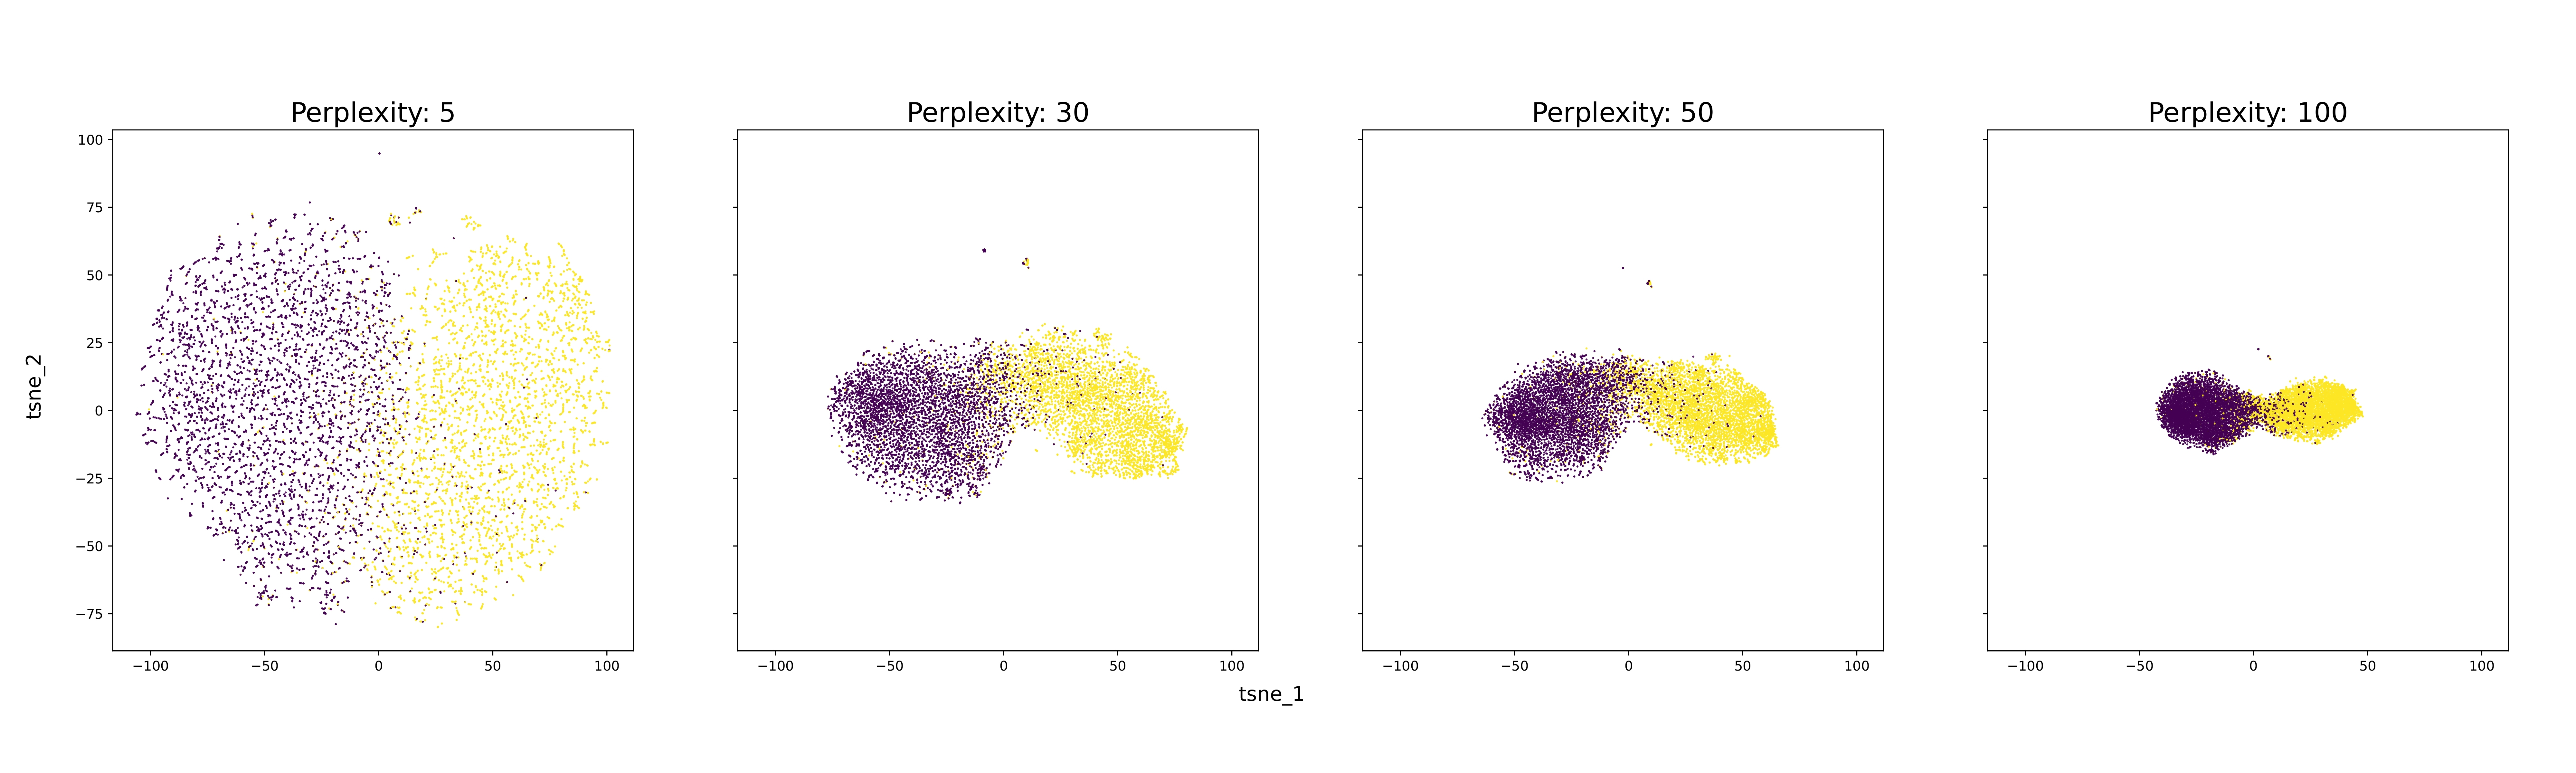
\includegraphics[width=1\textwidth]{img/reductions-mr-1000.jpg}
    \caption{t-SNE reductions with various perplexity values after 1,000 iterations performed on the embedded and normalized Movie Review dataset.}
    \label{fig:reductions-mr-1000}
\end{figure}

\begin{figure}[htbp]
    \centering
    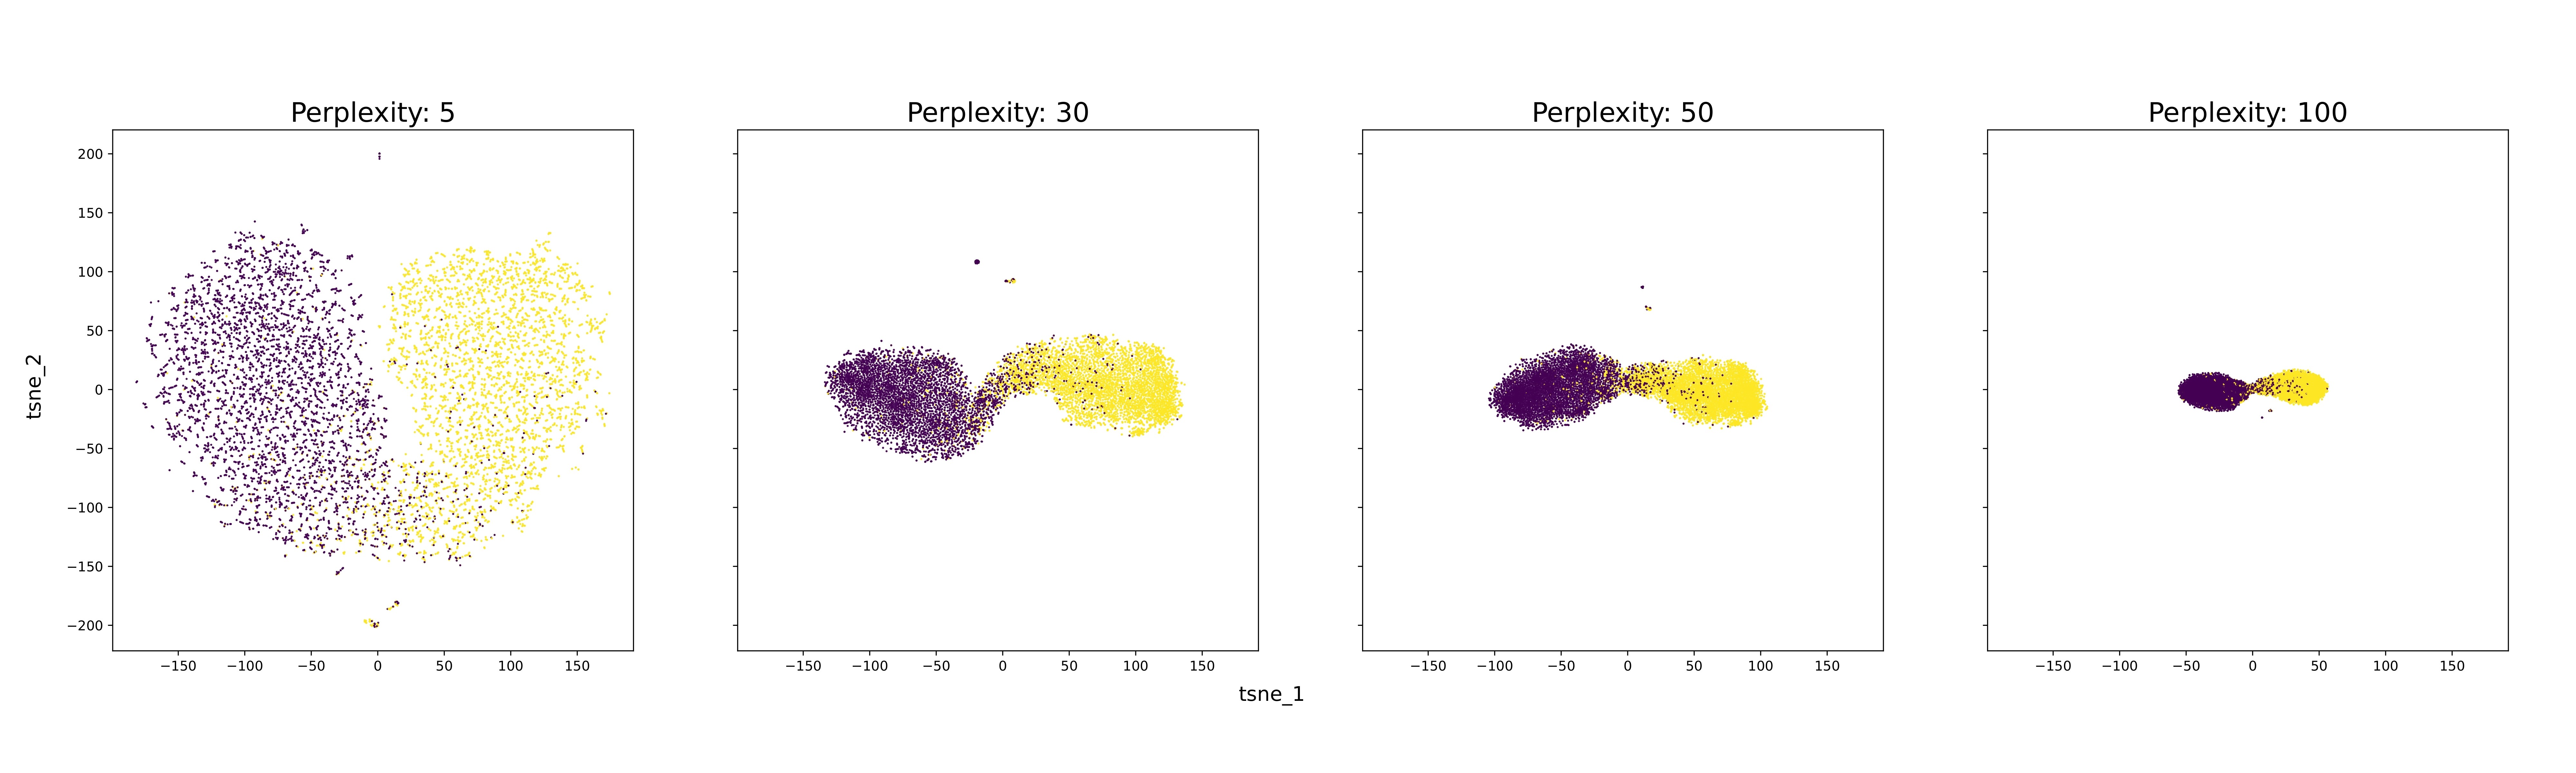
\includegraphics[width=1\textwidth]{img/reductions-mr-5000.jpg}
    \caption{t-SNE reductions with various perplexity values after 5,000 iterations performed on the embedded and normalized Movie Review dataset.}
    \label{fig:reductions-mr-5000}
\end{figure}

\begin{figure}[htbp]
    \centering
    \includegraphics[width=1\textwidth]{img/reductions-ag-news-1000.jpg}
    \caption{t-SNE reductions with various perplexity values after 1,000 iterations performed on the embedded and normalized AG's News dataset.}
    \label{fig:reductions-agnews-1000}
\end{figure}

\begin{figure}[htbp]
    \centering
    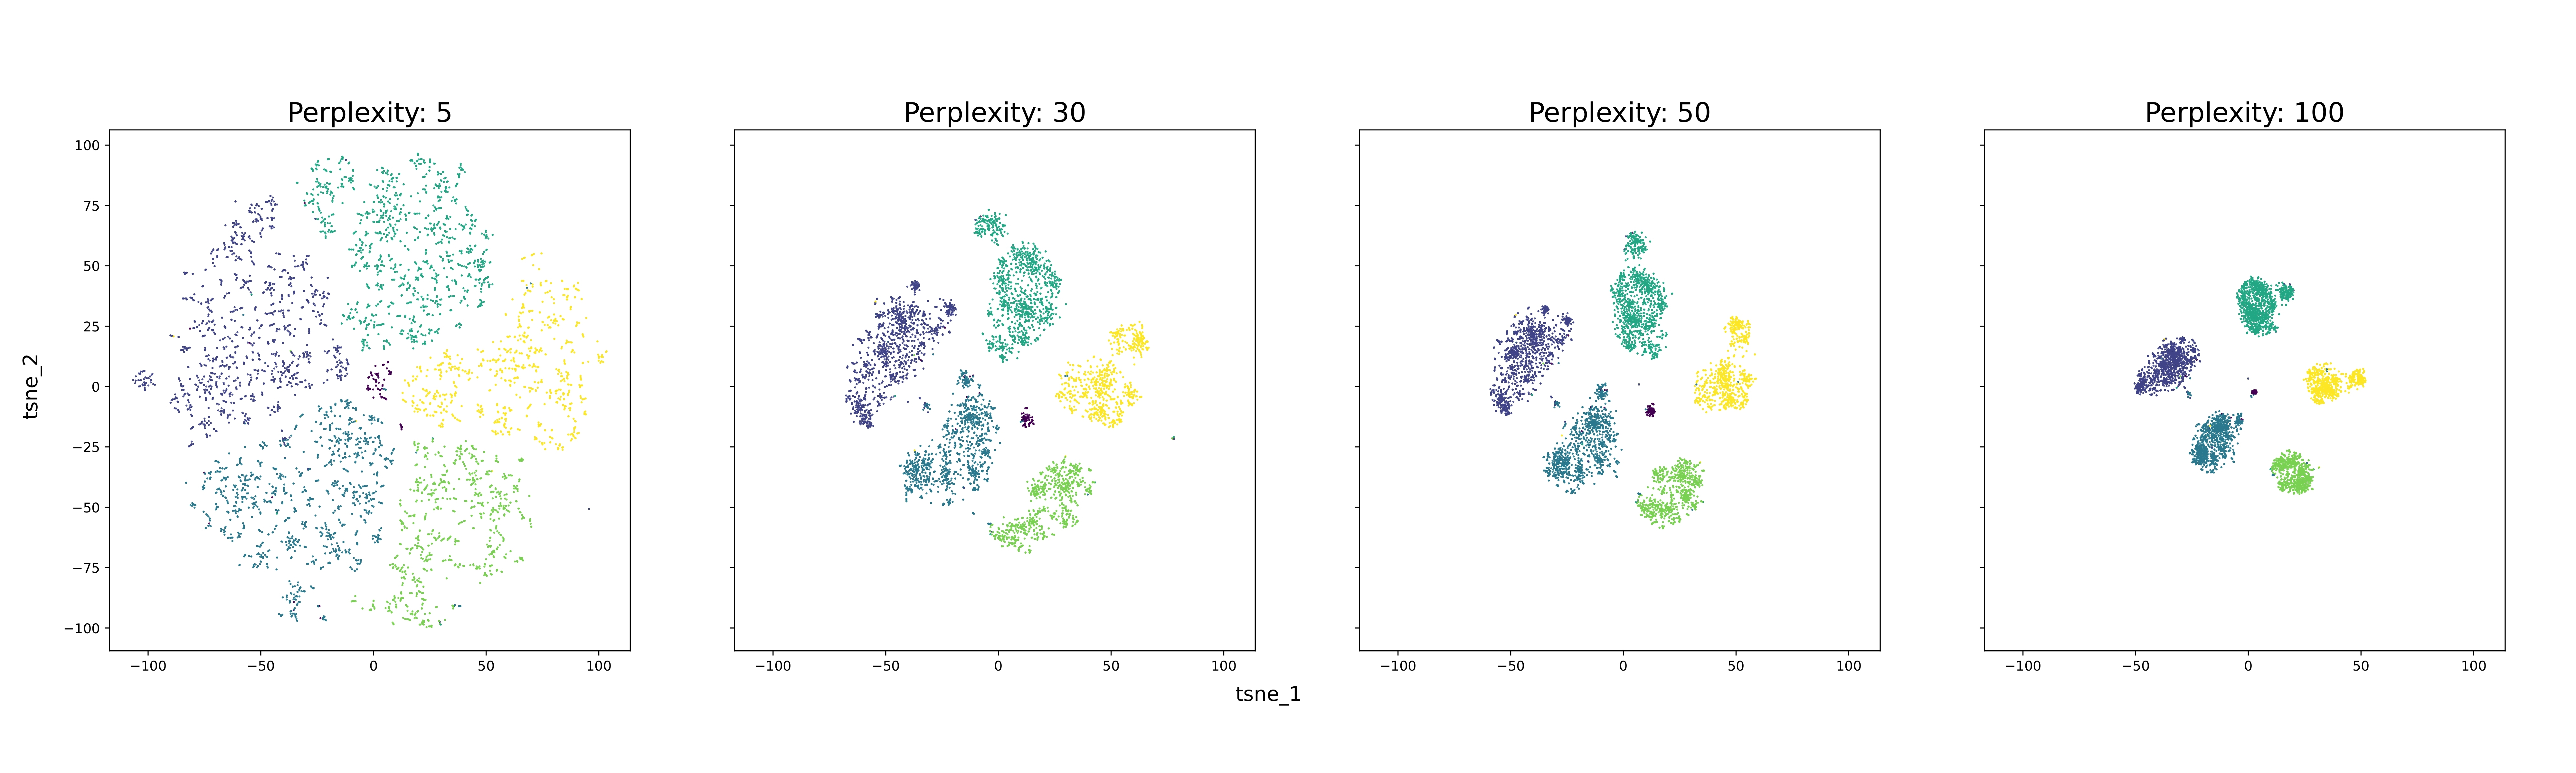
\includegraphics[width=1\textwidth]{img/reductions-trec-1000.jpg}
    \caption{t-SNE reductions with various perplexity values after 1,000 iterations performed on the embedded and normalized TREC-6 dataset.}
    \label{fig:reductions-trec-1000}
\end{figure}

\fi

% Starting at a perplexity of 30, the points begin to cluster more and more tightly. The clusters do not seem to separate in any of the runs -- it is important to note, however, that distances and sizes of the clusters do necessarily carry any meaning when examining the reduction plots (\cite{wattenberg2016how}, \cite{vanHomepage}).

% It is also worth noting that the differences between 1,000 and 5,000 iterations appear quite small despite the relative increase in computations. \dots

I selected two state-of-the-art transformers, BERT (\cite{DBLP:conf/naacl/DevlinCLT19}) and SetFit (\cite{DBLP:setfit}) to fine-tune as models for this experiment. BERT is an established language model pre-trained on 3,300M english words. It uses bidirectional self-attention in order to incorporate context from both directions of a given token, unlike many previous context-sensitive approaches which only considered a single direction. For this experiment, I will be using BERT\textsubscript{BASE}, which consists of 12 layers, hidden units of size 768 with 110M parameters in total. SetFit, on the other hand, is based on sentence transformers (\cite{DBLP:conf/emnlp/ReimersG19}) which are then fine-tuned in a contrastive manner. This model is similarly made up of 12 layers and generates 768-dimensional embeddings, but has a parameter count of 109M.  

The experiment is conducted by performing 20 queries on 25 instances, with a validation set size of 10\%. The results will be averaged over five runs of queries per combination of dataset, model and query strategy. The training and evaluation of these models is run using an AL experiment setup based on the Python library Small-Text (\cite{schroeder2023small-text}).

Alongside the original Core-Set (CS), I will be comparing my different approaches with Random Sampling (RS) and Breaking-Ties (BT). RS offers a good view of a baseline performance and will be interesting when compared to Core-Set. BT, on the other hand, may serve as a good upper bound when looking at improving Core-Set's performance.

\section{Experiment Results}

% Based on the experimental setup outlined in Section 4.2, this chapter presents the outcomes for each experiment run. Section 4.3.1 will show the learning curves for the each training run, and Section 4.3.2 will report on the corresponding result tables.
Based on the experimental setup outlined in Section 4.2, this chapter presents the outcomes for each experiment run. I first present the learning curves for the each training run, then report on the corresponding result tables.

\iffalse
%% TEMPLATE TABLE
\begin{table*}[h!]%
\centering
\fontsize{8pt}{9pt}\selectfont%
\renewcommand{\tabcolsep}{12pt}%
\begin{tabular}{@{}ll@{\hspace{10pt}} r @{${}\pm{}$} r r @{${}\pm{}$} r r @{${}\pm{}$} r r @{${}\pm{}$} r @{}}
\toprule
\textbf{Dataset} & \textbf{Model} & \multicolumn{8}{c}{\textbf{Query Strategy}}\\
\cmidrule{3-10} & & \multicolumn{2}{c}{\hspace*{-6pt}RS} & \multicolumn{2}{c}{BT} & \multicolumn{2}{c}{CS} & \multicolumn{2}{c}{\hspace*{4pt}Unknown}\\
\midrule
\multirow{2}{*}{AGN}  & BERT & 1.852 & 0.415 & 0.907 & 0.203 & \bfseries 0.432 & \bfseries 0.097 & 516.554 & 115.583 \\
 & SetFit & 7.264 & 1.626 & \bfseries 6.199 & \bfseries 1.389 & 10.256 & 2.359 & 481.758 & 142.013 \\
\midrule
\multirow{2}{*}{MR}  & BERT & 0.014 & 0.003 & 0.014 & 0.003 & \bfseries 0.009 & \bfseries 0.002 & 1.889 & 0.425\\
 & SetFit & 0.521 & 0.117 & \bfseries 0.436 & \bfseries 0.098 & 0.468 & 0.105 & 3.672 & 1.098 \\
\midrule
\multirow{2}{*}{TREC-6}  & BERT & 0.085 & 0.019 & 0.042 & 0.009 & \bfseries 0.018 & \bfseries 0.004 & 0.609 & 0.138 \\
 & SetFit & 0.289 & 0.065 & \bfseries 0.248 & \bfseries 0.055 & 1.111 & 0.745 & 1.504 & 0.447 \\
\bottomrule
\end{tabular}
\caption{%
Final accuracy per dataset, model, and query strategy. We report the mean and standard deviation over five runs. The best result per dataset is printed in bold.}
\label{table-results-acc}
\end{table*}
\fi

% \subsection{Learning Curves}

The following figures show the learning curves for each combination of dataset, model and query strategy. 

\clearpage \newpage

\begin{figure}[htbp]
    \centering
    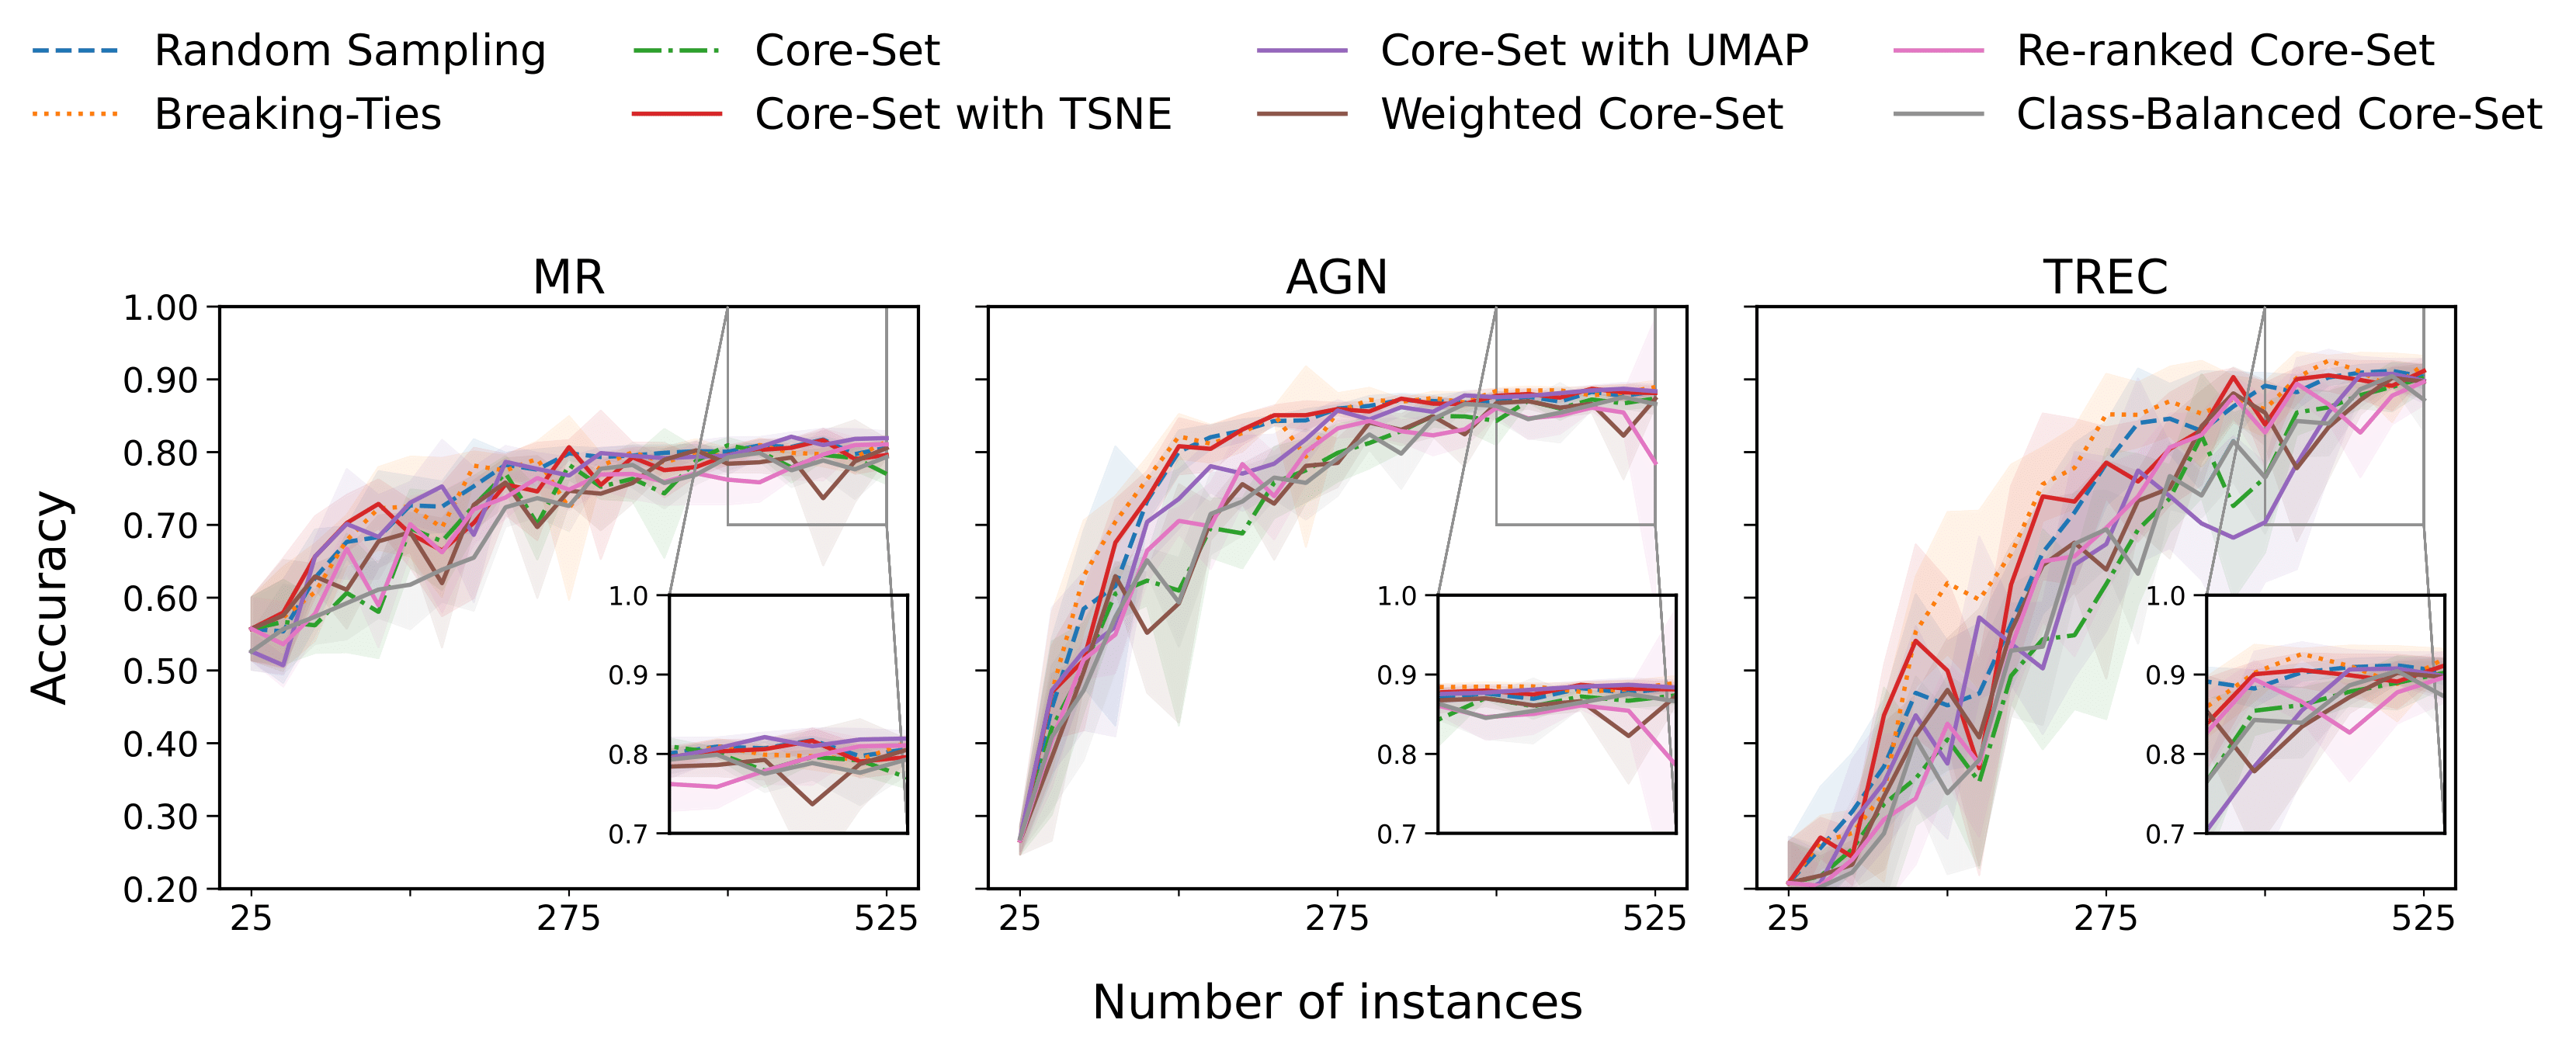
\includegraphics[width=1\textwidth]{img/bert-plots-1.png}
    \caption{Active Learning curves of BERT on each dataset when combined with seven query strategies: Random Sampling, Breaking-Ties, Core-Set, Core-Set with t-SNE, Core-Set with UMAP, Weighted Core-Set, Re-ranked Core-Set and Class-Balanced Core-Set. The lines represent the mean accuracy and the surrounding tubes represent the standard deviation over five runs.}
    \label{fig:bert-curves}
\end{figure}

\begin{figure}[htbp]
    \centering
    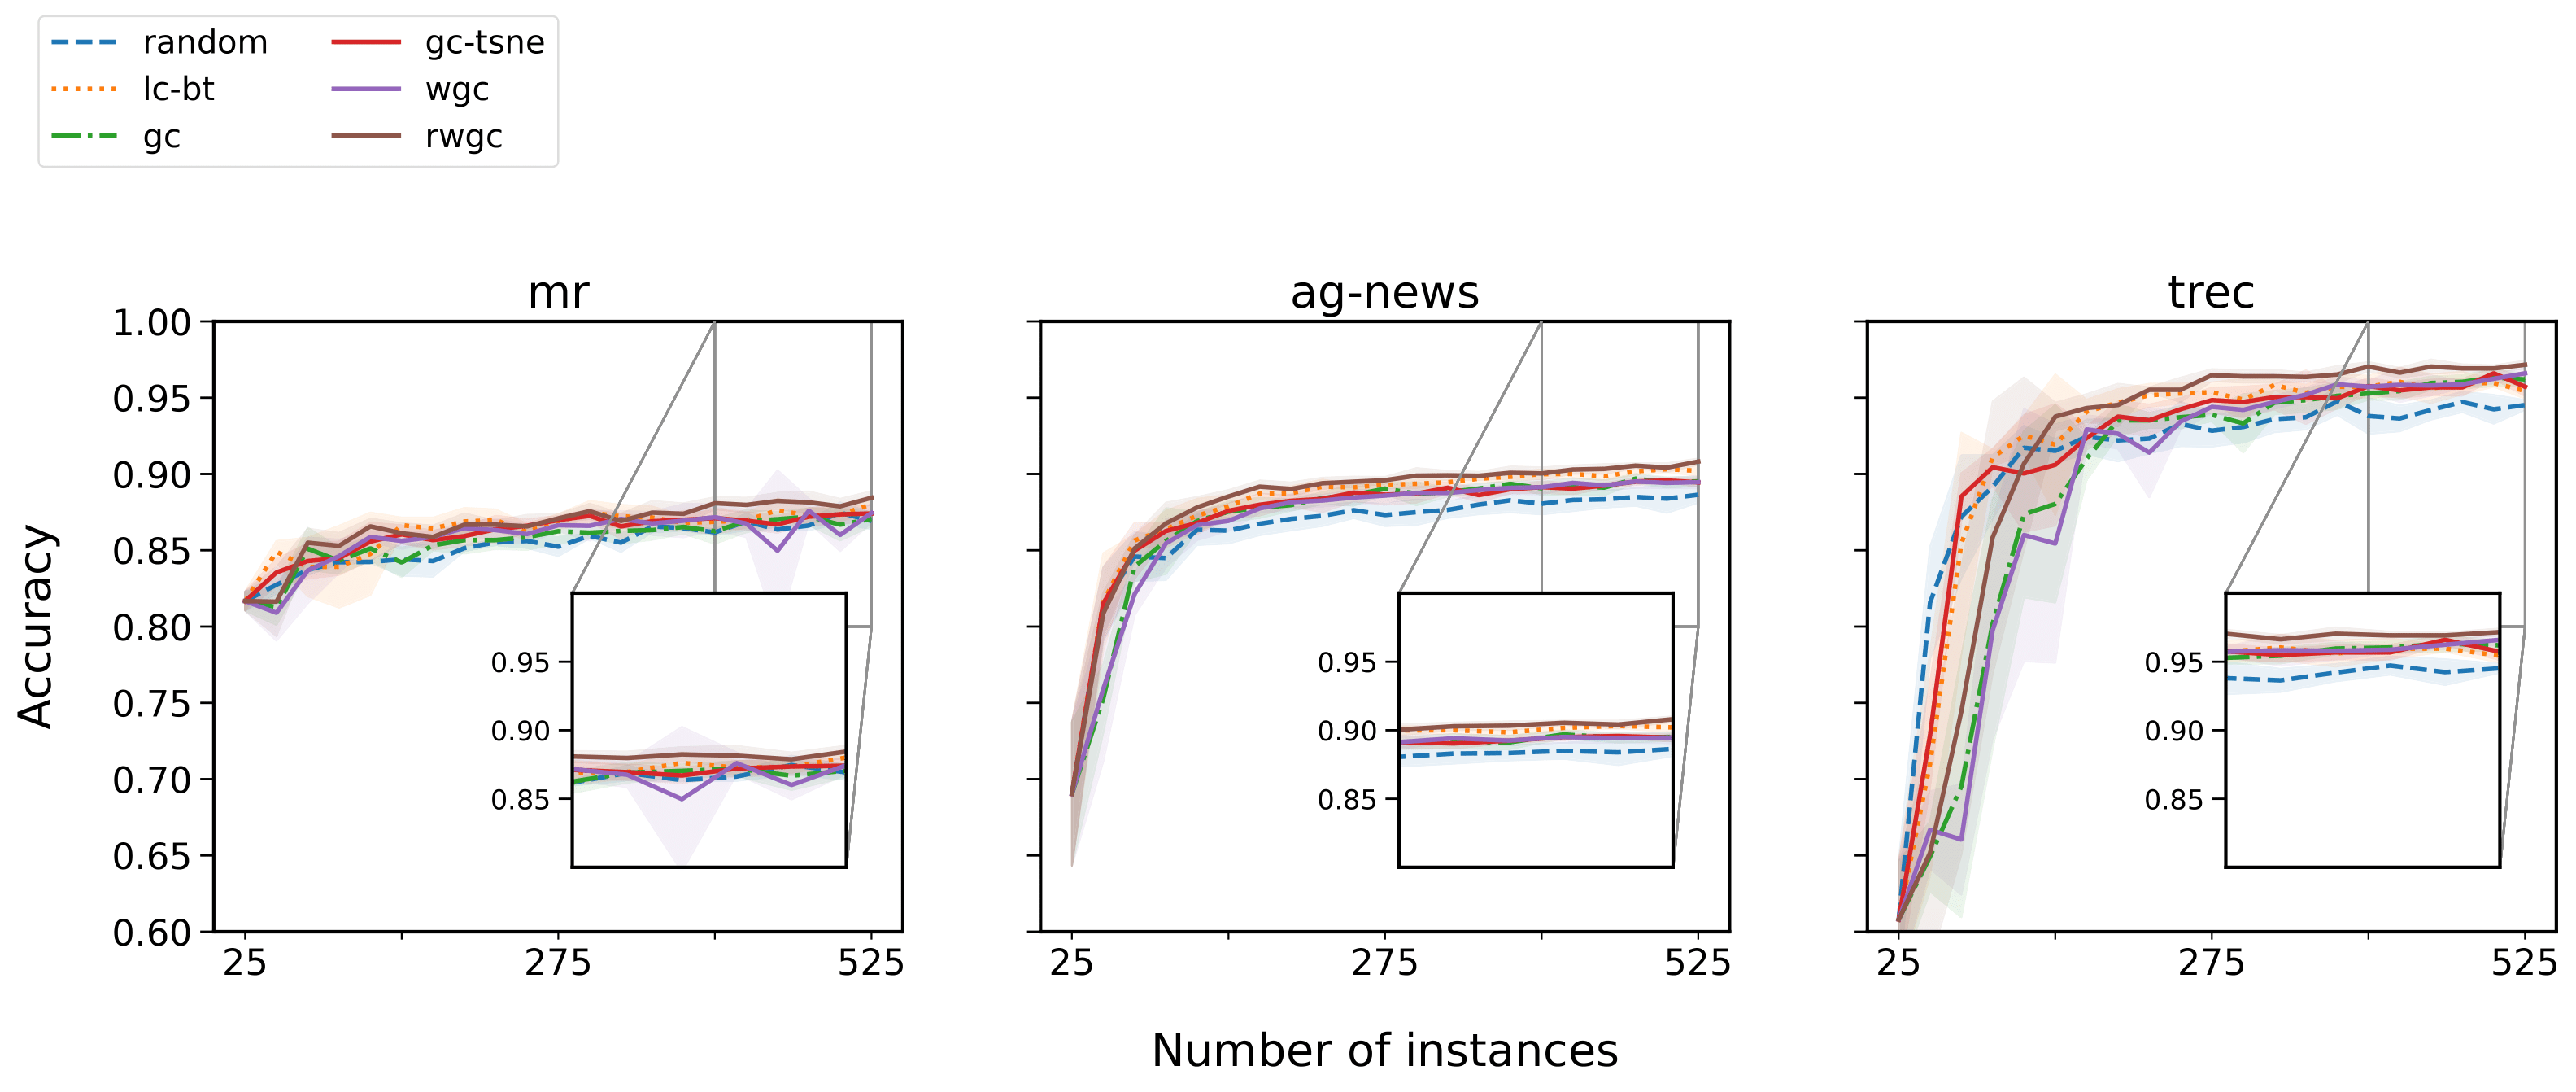
\includegraphics[width=1\textwidth]{img/setfit-plots-1.png}
    \caption{Active Learning curves of SetFit on each dataset when combined with eight query strategies: Random Sampling, Breaking-Ties, Core-Set, Core-Set with t-SNE, Core-Set with UMAP, Weighted Core-Set, Re-ranked Core-Set and Class-Balanced Core-Set. The lines represent the mean accuracy and the surrounding tubes represent the standard deviation over five runs.}
    \label{fig:setfit-curves}
\end{figure}

\clearpage

% GENERAL: Comparing models
Overall, the SetFit learning curves generally outperform the BERT model and seem to show much less variation between the different query strategies. This is reflected not only in the mean curve progressions of each model, but also in the smaller standard deviations of each individual line. Even in the case of BERT's resulting AL curves, the most noticeable accuracy differences seem to mainly occur in early iterations. Generally, the mean accuracy scores of the different strategies tend to lie in a similar range by the final iteration. 

I will first compare and contrast the different results for the training of the BERT model (Figure ~\ref{fig:bert-curves}). We can clearly see general upwards trends to varying degrees depending on the dataset. The highest final accuracies are achieved on the TREC dataset, whereas the learning curves for AGN have the fastest increase in early iterations. Both seem to resemble a saturation curve, with TREC's mean accuracy values starting to slowly level out around 90\%, whereas AGN's stop around 85\% near the second half of the learning process. From this point on, the curves of both datasets gradually rise by around 5\% towards the end of training. On the other hand, the learning curves on MR show a more gradual, steady rise throughout the entire process and finish with slightly lower overall accuracies, with all results coming out to just under or around 80\%. 

% BERT: comparing query strategies
When comparing the curves of the different query strategies, we can see that specifically in the case of BERT, CS does indeed seem to underperform when compared to the baseline approaches. This is mainly noticeable when looking at the earlier iterations (between queries 1 to 10). The underperformance of CS becomes even more apparent when considering the fact that the learning curves of RS are consistently above those of CS. This further reinforces the sentiment that Core-Set may have weaknesses within the domain of text classification. 

In the case of AGN and TREC, we can clearly see the curve of BT achieve high performances throughout, although CS-tSNE is able to compete very closely on AGN. Interestingly enough, RS has managed to achieve similar scores to the strategies mentioned previously in these cases.

We also observe that in most cases, the different variations of Core-Set seem to be on par with or more performant than the original Core-Set. Especially CS-tSNE looks to be a strong contender in all cases and manages to perform similarly to or better than Core-Set and the remaining variants. 

CS-UMAP also performs favorably, especially in the case of MR, where it remains on the upper end of accuracy scores throughout and manages to outperform all other strategies by the final iteration. In the case of AGN and TREC, we still find improvements to Core-Set during training, although these datasets seem to generally favour the t-SNE approach. Interestingly, the learning curve takes a dip in the latter half of training on the TREC dataset and rises rapidly again in the final iterations. Notably, a comparable sharp decrease is apparent in the first half of training on the same dataset for CS-tSNE's curve.

The class-balanced approach, on the other hand, does not seem to show significant accuracy improvements during training in comparison to the regular Core-Set approach. One discernible difference with the learning curve of CB-CS is noticeable on the MR dataset, where its curve seems to have much less fluctuations than CS and its other variations. Generally, however, CS and its class-balanced version show very similar learning curve trends across all three datasets. 

Weighted Core-Set and Re-ranked Core-Set are in a similar vein to, albeit oftentimes slightly above, the Class-Balanced approach. Both curves fluctuate around the same level or slightly higher than CS, but do not manage to surpass the baseline approaches in early iterations. We can see that in the case of AGN, the re-ranked strategy's learning curve even takes a dip in mean accuracy towards the end, resulting in a mean final accuracy below that of all other strategies by the final iteration despite being relatively competitive in prior iterations.

% SetFit: comparing datasets
The SetFit learning curves (Figure ~\ref{fig:setfit-curves}) show much less fluctuation throughout the individual learning curves, as well as smaller discrepancies between the different query strategies during training. 

In the case of MR, all strategies have very similar accuracy curves and bundle tightly around the final iterations, with all final values somewhere around 87,5\%. For this dataset, the increase throughout the entire process is very minimal, amounting to only around 5\% from the first query to the end of training. As for AGN and TREC, more learning progress is visible from beginning to end. Moreover, the margins between the curves are slightly wider, and some differences can be noted when comparing the different strategies. For these two datasets, the curves again show large early increases around the first five iterations, with the values starting to level out somewhere between instance 150 and 275. For these datasets, the values by the last iteration are also higher than for MR, with final results around the 90\% mark on AGN and around 95\% on TREC.

% SetFit: comparing query strategies
Again, BT stands out as one of the best strategies, with CS-TSNE generally following a similar trend. In contrast to BERT, CS itself does not seem to underperform throughout in any significant way. Only in the first half of the learning process on TREC can we see some kind of noticeable difference between CS and the other curves. In these earlier instances, CS is outperformed by the baseline strategies as well as the dimensionality reduction-based strategies. 

In this diagram we can also observe the different strategies fall into two ``groups'' of curve progressions in the beginning iterations. Similarly to Figure~\ref{fig:bert-curves}, we can see WCS, RCS and CB-CS following a very close trend to that of CS. The other query strategies (RS, BT, CS-tSNE, CS-UMAP) seem to follow a slightly higher, but similarly bundled, trend. This bundling of query strategies is only noticeable on the TREC dataset curves, whereas the other graphs seem to show all or most strategies bundled closer together overall.

One slight outlier in these graphs is RS, of which the accuracy values stay visibly below the other query strategies in the second half of each run, specifically when considering AGN and TREC. For these two datasets, RS seems to be competitive in early iterations, outperforming CS and many of the other strategies, but progress rapidly slows, resulting in lower final scores than the other strategies.

% \subsection{Tables}

The following page shows two tables containing the mean accuracy (Table~\ref{table-results-acc}) and mean AUC values (Table~\ref{table-results-auc}) corresponding to the learning curves. 

\clearpage \newpage

% NEW TABLES
\begin{sidewaystable}[htpb]

\centering
\fontsize{8pt}{9pt}\selectfont%
\renewcommand{\tabcolsep}{6pt}%
\begin{tabular}{@{}ll@{\hspace{10pt}} r @{${}\pm{}$} r r @{${}\pm{}$} r r @{${}\pm{}$} r r @{${}\pm{}$} r r @{${}\pm{}$} r r @{${}\pm{}$} r r @{${}\pm{}$} r r @{${}\pm{}$}r @{}}
\toprule
\textbf{Dataset} & \textbf{Model} & \multicolumn{14}{c}{\textbf{Query Strategy}}\\
\cmidrule{3-18} & & \multicolumn{2}{c}{\hspace*{-6pt}RS} & \multicolumn{2}{c}{BT} & \multicolumn{2}{c}{CS} & \multicolumn{2}{c}{\hspace*{4pt}CS-TSNE} & \multicolumn{2}{c}{\hspace*{4pt}CS-UMAP} & \multicolumn{2}{c}{\hspace*{4pt}WCS} & \multicolumn{2}{c}{\hspace*{4pt}RCS} & \multicolumn{2}{c}{\hspace*{4pt}CS-CB} \\
\midrule

\multirow{2}{*}{AGN}  & BERT & 0.884 & 0.004 &  \bfseries 0.889 & \bfseries 0.010 & 0.874 & 0.012 & 0.881 & 0.010 & 0.884 & 0.010 & 0.873 & 0.011 & 0.785 & 0.221 & 0.866 & 0.016\\ 
 & SetFit & 0.886 & 0.006 & \bfseries 0.902 & \bfseries 0.004 & 0.895 & 0.003 & 0.895 & 0.003 & 0.899 & 0.001 & 0.895 & 0.005 & 0.895 & 0.004 & 0.898 & 0.006 \\
 
\multirow{2}{*}{MR}  & BERT & 0.806 & 0.011 & 0.815 & 0.009 & 0.770 & 0.015 & 0.796 & 0.020 & \bfseries 0.819 & \bfseries 0.011 & 0.806 & 0.014 & 0.811 & 0.013 & 0.793 & 0.021\\ 
 & SetFit & 0.869 & 0.006 & \bfseries 0.880 & \bfseries 0.005 & 0.871 & 0.005 & 0.874 & 0.005 & 0.876 & 0.008 & 0.874 & 0.007 & 0.870 & 0.004 & 0.870 & 0.006 \\

\multirow{2}{*}{TREC}  & BERT & 0.904 & 0.018 & \bfseries 0.920 & \bfseries 0.014 & 0.902 & 0.021 & 0.912 & 0.009 & 0.898 & 0.033 & 0.897 & 0.027 & 0.897 & 0.036 & 0.872 & 0.048\\ 
 & SetFit & 0.945 & 0.004 & 0.954 & 0.006 & 0.962 & 0.004 & 0.957 & 0.007 & 0.962 & 0.010 & \bfseries 0.966 & \bfseries 0.004 & 0.962 & 0.003 & 0.956 & 0.007 \\
 
\bottomrule
\end{tabular}

\caption{%
Final accuracy per dataset, model, and query strategy. We report the mean and standard deviation over five runs. The best result per dataset is printed in bold.}
\label{table-results-acc}

\vspace{2\baselineskip}

\centering
\fontsize{8pt}{9pt}\selectfont%
\renewcommand{\tabcolsep}{6pt}%
\begin{tabular}{@{}ll@{\hspace{10pt}} r @{${}\pm{}$} r r @{${}\pm{}$} r r @{${}\pm{}$} r r @{${}\pm{}$} r r @{${}\pm{}$} r r @{${}\pm{}$} r r @{${}\pm{}$} r r @{${}\pm{}$} r @{}}
\toprule
\textbf{Dataset} & \textbf{Model} & \multicolumn{14}{c}{\textbf{Query Strategy}}\\
\cmidrule{3-18} & & \multicolumn{2}{c}{\hspace*{-6pt}RS} & \multicolumn{2}{c}{BT} & \multicolumn{2}{c}{CS} & \multicolumn{2}{c}{\hspace*{4pt}CS-TSNE} & \multicolumn{2}{c}{\hspace*{4pt}CS-UMAP} & \multicolumn{2}{c}{\hspace*{4pt}WCS} & \multicolumn{2}{c}{\hspace*{4pt}RCS} & \multicolumn{2}{c}{\hspace*{4pt}CS-CB}\\
\midrule
 
\multirow{2}{*}{AGN}  & BERT & 0.790 & 0.015 & \bfseries 0.800 & \bfseries 0.009 & 0.735 & 0.020 & 0.792 & 0.007 & 0.772 & 0.019 & 0.731 & 0.014 & 0.741 & 0.015 & 0.733 & 0.017\\ 
 & SetFit & 0.865 & 0.007 & \bfseries 0.881 & \bfseries 0.004 & 0.871 & 0.005 & 0.875 & 0.004 & 0.879 & 0.004 & 0.870 & 0.003 & 0.870 & 0.002 & 0.873 & 0.003 \\

\multirow{2}{*}{MR}  & BERT & \bfseries 0.750 & \bfseries 0.007 & 0.746 & 0.011 & 0.718 & 0.009 & 0.741 & 0.017 & 0.748 & 0.005 & 0.720 & 0.004 & 0.718 & 0.005 & 0.706 & 0.015\\ 
 & SetFit & 0.854 & 0.002 & \bfseries 0.864 & \bfseries 0.005 & 0.856 & 0.003 & 0.862 & 0.003 & 0.866 & 0.005 & 0.858 & 0.007 & 0.857 & 0.003 & 0.859 & 0.002 \\
 
\multirow{2}{*}{TREC}  & BERT & 0.674 & 0.029 & \bfseries 0.709 & \bfseries 0.008 & 0.594 & 0.022 & 0.676 & 0.037 & 0.609 & 0.029 & 0.629 & 0.024 & 0.624 & 0.012 & 0.598 & 0.025\\ 
 & SetFit & 0.914 & 0.011 & \bfseries 0.923 & \bfseries 0.007 & 0.896 & 0.015 & 0.919 & 0.005 & 0.921 & 0.008 & 0.893 & 0.012 & 0.897 & 0.012 & 0.905 & 0.010 \\

 
\bottomrule
\end{tabular}

\caption{Final AUC per dataset, model, and query strategy. We report the mean and standard deviation over five runs. The best result per dataset is printed in bold.}
\label{table-results-auc}

\end{sidewaystable}

\clearpage

% Accuracy Table
%In Table~\ref{table-results-acc}, I show the reported mean final accuracy across all runs, as well as the standard deviation for each combination of dataset, model and query strategy. 

%Overall, Breaking-Ties dominates for almost every dataset on both models. Only for SetFit does another strategy achieve the highest overall final mean accuracy. Furthermore, we can see that RS outperforms CS when used with BERT throughout all datasets.

In Table~\ref{table-results-acc}, BT dominates for almost every dataset on both models. Only in two cases does another strategy achieve the highest overall final mean accuracy. Even though the differences are predominantly characterized by very small margins throughout, there are still noteworthy observations to be made.

First, we can again see that RS outperforms CS when used with BERT throughout all datasets. CS seems to encounter minor difficulties specifically on the MR dataset with BERT, where it marks the lowest result of all the strategies. Despite this, CS' training with the SetFit model yields improved results, particularly when contrasted with those achieved by RS with SetFit.

The results of the CS variations show small improvements in accuracy at various points. CS-tSNE and CS-UMAP most notably show slightly higher scores than CS in almost all cases. For CS-tSNE, the only exception is on TREC with SetFit. This row of results has some other noteworthy differences between query strategies. We can see that is the only combination of model and dataset for which CS, along with all of its variations, scores a higher result than BT. In the case of CS-UMAP, the only instance where we find no improvement to CS is on the TREC dataset. However, we observe quite consistent accuracy scores above 80\% for this strategy across the board. Additionally, this approach manages to improve upon Core-Sets relatively low accuracy score on the MR dataset with BERT, increasing from 77\% to nearly 82\%.

Although WCS does have the best result in the case of the TREC dataset with SetFit, the remaining results in its column do not show consistent improvements when compared to CS. A similar sentiment applies to RCS and CS-CB, whose results in comparison to CS seem to be a mixed bag. 

Even so, all of the CS variations also show some kind of improvement in the case of MR with BERT, in which CS has the lowest accuracy overall. Notably, AGN is the only dataset where CS-TSNE, WCS and RCS do not have any impact on the accuracy score in the case of SetFit. Even in cases where results are not exactly the same, they often remain within a one-standard-deviation range of each other. One row where this is most evident is the combination of SetFit and MR across all query strategies.

% AUC Table
Table~\ref{table-results-auc} contains the reported mean AUC (area under curve) and the corresponding standard deviation for each combination of dataset, model and query strategy. The top performing AUC results, similarly to the accuracy table, show BT as having the best results in almost all cases. Unexpectedly, RS manages to reach the highest AUC among all query strategies in the case of MR with BERT.

Again, the CS variations offer some minor improvements in many cases. Here, the similarity between the curves of CS, WCS, RCS and CB-CS becomes more apparent, as the values of these strategies are almost equal in most cases. Nonetheless, CS-TSNE shows higher AUC values than CS across the board. The largest improvement was achieved with BERT, namely on TREC (8.2\%), with the second largest being on MR (5.7\%).

\chapter{Discussion}

% INTRODUCTION
Although none of the proposed Core-Set variations manage to get scores consistently as high as the Breaking-Ties approach, we can still gather interesting insights from the conducted experiment. 

% ANSWERING RESEARCH QUESTIONS?
One presumption prior to the conducting of the experiment was that Core-Set may have mixed results in cases of text classification. Not only that, but according to \cite{DBLP:conf/kdd/0002MM21}, Core-Set's results with BERT sometimes lie even below the performance of Random Sampling. This experiment's results further support this statement, with Core-Set being outperformed by Random Sampling with BERT, both in accuracy and AUC.

In order to discuss the research questions posed in Chapter 1, I have structured the rest of this chapter according to the results of each approach presented in Chapter 3. Pertaining to the third research question, I have also conducted further analysis of the experiment results in order to determine whether the approach did indeed result in a more balanced distribution of classes in the labelled pool.

\section{Dimensionality Reduction-Based Approach}

The experiment has also offered further insights with regard to the research questions. The first modification to Core-Set, which used t-SNE to reduce word embeddings prior to the selection with k-Center greedy, generally managed to improve Core-Set over the three given datasets. Though the differences in the case of SetFit were very minor, we can observe more noticeable improvements in efficiency with BERT, where Core-Set seemed to have its weaknesses originally.  

\section{Uncertainty-Based Approach}

In the case of the two attempts to combine an uncertainty-based approach with Core-Set, the results have shown minor, but generally insignificant improvements. Though WCS and RCS had generally similar results overall, the results are still slightly in favour of WCS due to the improvements on TREC with SetFit and AGN with BERT, in which RCS fell short. Another aspect that favours WCS over RCS is the ease of implementation and interpretability, which is very straightforward in the case of the weighted approach. In addition, WCS does not perform what are essentially two instance selection runs per query, which is the case in the re-ranked approach.

\section{Class Balance-Based Approach}

Finally, with regard to the third research question, it becomes clear that the proposed class balance-based approach does not manage to improve upon the Core-Set selection. The accuracy and AUC values are, in most cases, either on par with or slightly below those of Core-Set.

In order to investigate the functionality of the class-balanced approach, I tracked the class distributions after each query of the previously conducted experiment. As a result, I was able to observe an overall positive impact of the balancing on the class distribution within the labelled pool. This impact was measured using the normalized entropy within the labelled pool after each iteration, as explained in Chapter 3. Similar to the learning curves in Chapter 4, I have plotted the mean over five runs in Figure~\ref{fig:entropy-plot}. 

\begin{figure}[htbp]
    \centering
    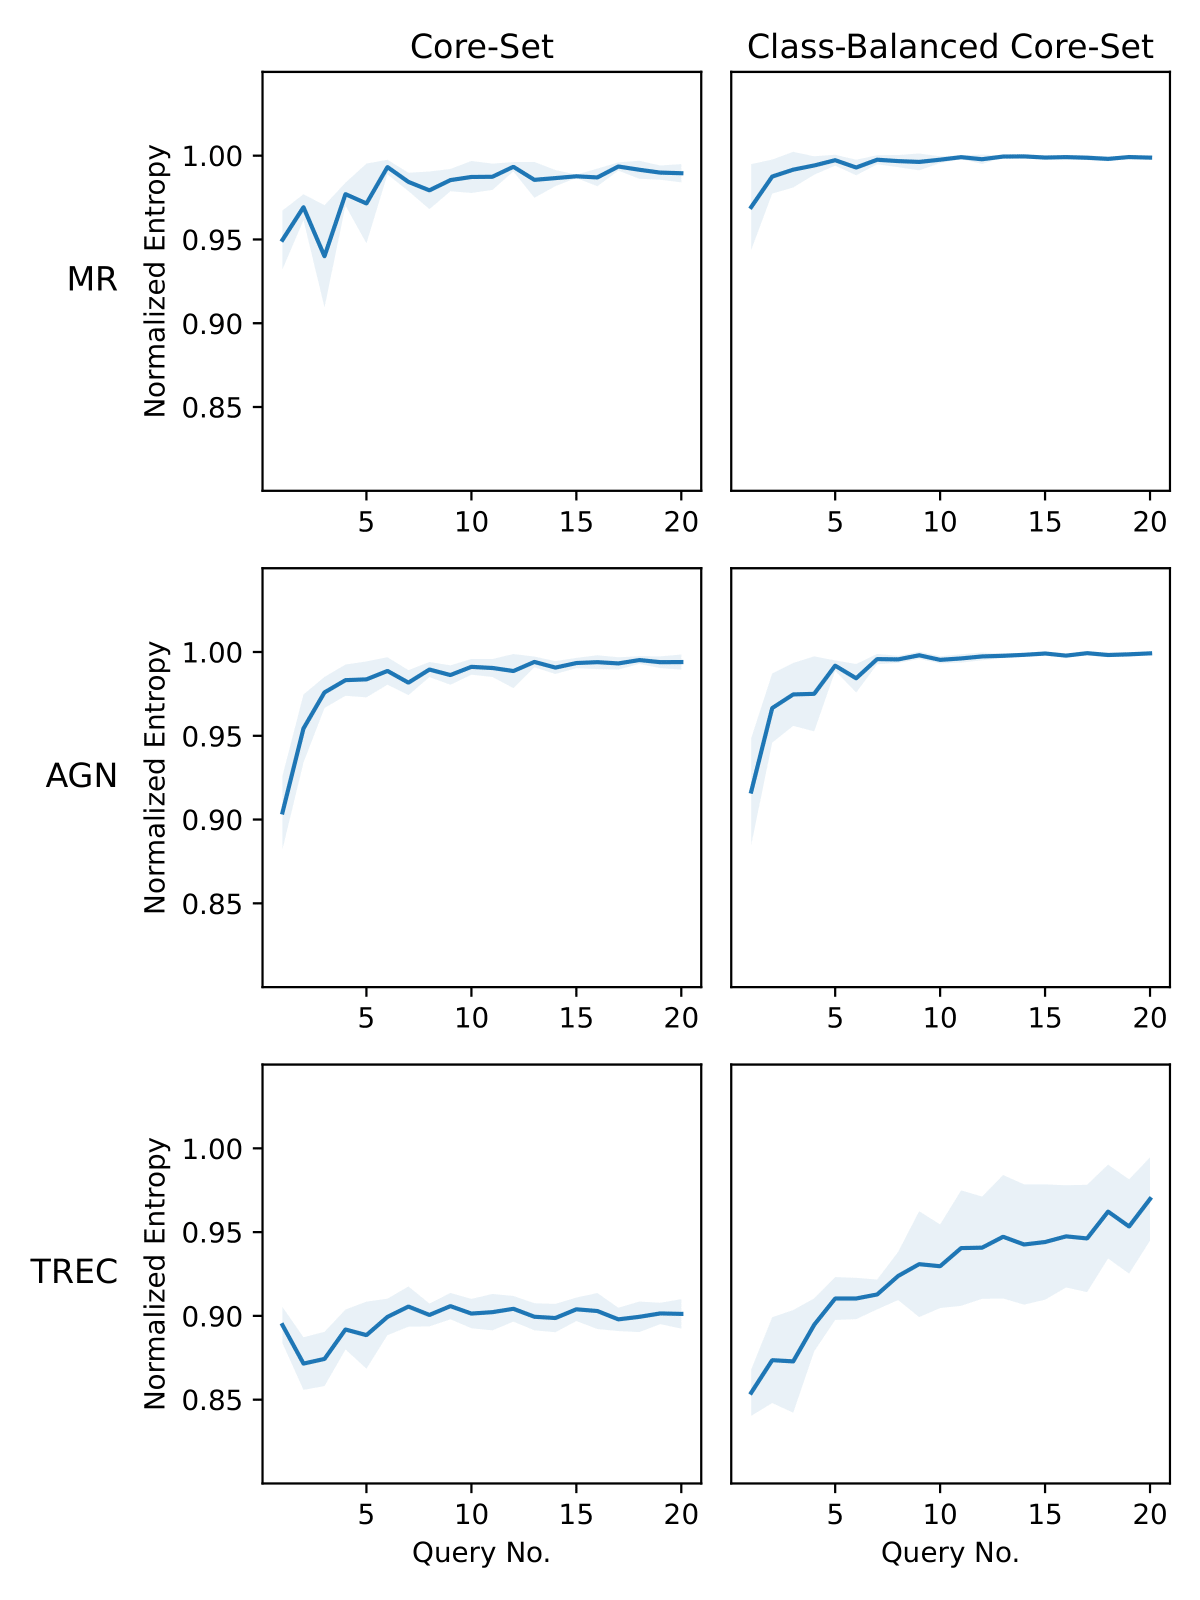
\includegraphics[scale=0.6]{img/entropy_plots-1.png}
    \caption{Normalized entropy curves for instances selected during AL with BERT using Core-Set and Class-Balanced Core-Set. The lines represent the mean accuracy and the surrounding tubes represent the standard deviation over five runs.}
    \label{fig:entropy-plot}
\end{figure}

We can see that for both strategies, the normalized entropy generally increases or stays relatively constant with each query. In the case of MR, we observe only minor changes in the class distribution throughout the learning process. This may be in part attributed to the fact that this dataset only has two classes that are distributed evenly. Nonetheless, we observe the class-balanced approach to have a more stable mean normalized entropy in the first half of the learning process, whereas the regular Core-Set selection has slight fluctuations. Nevertheless, both curves run somewhere within the range of 0.95 and 1, indicating a very close to even distribution in both cases. 

For AGN, the difference between Core-Set and the class-balanced approach seem to be even less evident. In both cases, we observe a saturation curve beginning around 0.9 and evening out close to 1 around the fifth query. Although AGN has twice as many classes as MR, it is also a class balanced dataset with equal amounts of instances from each class, which may explain the depicted results.

The dataset in which a change in class distribution within the labelled pool is most distinct is TREC. Here, we note a relatively constant curve around or below a normalized entropy of 0.9 in the case of Core-Set, whereas the class-balanced approach manages to select an increasingly even distribution. In this case, the normalized entropy gradually rises from roughly 0.85 to around 0.97. Still, the standard deviation increases in later iterations, becoming clearly higher than in all other cases. 

One reason for these differences in the efficacy of the class-balanced approach are the underlying class distributions of each datast. In the case of MR and AGN, we have uniform distributions across all classes, whereas TREC is an inherently class-imbalanced dataset. Consequently, the class-balanced approach has very little impact on the distributions of the selected instances, which are nearly uniformally distributed in the first place. TREC, in contrast, has slightly imbalanced classes, resulting in the possibility for improvement using the class-balanced approach.

\section{Limitations}

Naturally, there are some limitations to consider with this experiment. On one hand, the training data used only encompassed three different datasets. These datasets do attempt to cover a variety of purposes, class numbers and sizes, but in order to further verify the effectiveness of the proposed approaches, more datasets should be used. 

Another aspect that was not considered by my experiment is the effect of each approach on the respective runtime. This may be especially relevant when considering a dimensionality reduction algorithm such as t-SNE, which could have a significant impact when training on larger datasets. Furthermore, this experiment's result evaluation only took into account the respective accuracy and AUC metrics. For the purpose of evaluating the results of each strategy, it may be worth considering other commonly used metrics such as the F1-score.

Finally, it is worth underlining the fact that this thesis examined Core-Set as the basic k-Center greedy approach, whereas \cite{DBLP:conf/iclr/SenerS18} propose a slightly optimized, robust k-Center approach that minimizes outliers. This approach was not used for implementation reasons, as the solution for robust k-Center's feasability check depends on Gurobi (\cite{gurobi}), a licensed optimization framework. As a result, the results of Core-Set and the corresponding modifications used in this experiment may not be optimal.

\section{Future Research}

As mentioned earlier, this experiment was conducted on three datasets, two of which have uniform class distributions. With regard to the class-balanced approach, it may be worth examining the effect on various datasets with more imbalanced class distributions. Not only may this result in more significant improvements in normalized entropy, but possibly some more noticeable changes for the learning process itself.

Furthermore, it could be worth investigating the affect of combining several of the approaches presented here. If two strategies such as CS-TSNE and CB-CS only offer minor improvements in some cases, maybe a combination of the two approaches could contribute to more efficient learning.

Of course, some of the aspects mentioned in the previous section could be added to this experiment for further research. Examining other metrics such as the F1-score and runtimes, as well as considering other classifiers and datasets may offer additional insights in determining the usability of the presented approaches. 

\chapter{Conclusion}

In this thesis, I examined the effect of Core-Set as an AL query strategy for text classification tasks and compared it with two baseline approaches using two models across three different datasets. I then created four different variations of Core-Set, each with some modification around the original k-Center greedy algorithm and examined their performance within the same experiment setup. The motivation for doing this was to see if Core-Set does indeed achieve mixed results within the field of text classification and to attempt to work toward a possible improvement in this regard.

The experiment's results show Core-Set producing mixed results in many cases when compared to the baseline strategies. This aligns with what can be observed in \cite{DBLP:conf/kdd/0002MM21}. We can observe some slight improvements of Core-Set's performances when used in conjunction with t-SNE. Moreover, the uncertainty-based approach and class balance-based approach do not seem to significantly impact Core-Set's results.

% \chapter*{Acknowledgements} % optional
% I thank the authors of the webisthesis template for their excellent work!

% \listoffigures % optional, usually not needed

% \listoftables % optional, usually not needed

% \listofalgorithms % optional, usually not needed
%    requires package algorithm2e

% optional: list of symbols/notation (e.g., using the nomencl package) but usually not needed

%\include{chapter1}
%\include{chapter2}

%\include{appendixA}

\appendix
\chapter{Implementation Details}

The experiment setup is based on a pre-existing AL environment created with \cite{schroeder2023small-text}. This also includes the implementation of k-Center greedy as well as various methods concerning class redistributions. In addition, well-known machine learning libraries such as Scikit-Learn, HuggingFace, NumPy, and SciPy were used for the implementation of the query strategies. These libraries were used within a Python 3.8 environment.

The models that were fine-tuned within the experiment are \href{https://huggingface.co/google-bert/bert-base-uncased}{bert-base-uncased} and \href{https://huggingface.co/sentence-transformers/paraphrase-mpnet-base-v2}{
paraphrase-mpnet-base-v2}. The datasets were also obtained via \href{https://github.com/huggingface/datasets}{huggingface datasets}.

% Bibliography
\bibliographystyle{plainnat} % requires package natbib. An alternative is apalike
\bibliography{literature}    % load file literature.bib

\end{document}
